\documentclass[12pt,a4paper]{ctexrep}
\usepackage{amsmath,amssymb}
\usepackage{fontspec}
\xeCJKsetup{AutoFallBack = true}
\setCJKfallbackfamilyfont\CJKrmdefault{Malgun Gothic}[Scale=MatchLowercase]
\setCJKfallbackfamilyfont\CJKsfdefault{Malgun Gothic}[Scale=MatchLowercase]
\setCJKfallbackfamilyfont\CJKttdefault{Malgun Gothic}[Scale=MatchLowercase]
\usepackage[top=1.5cm,bottom=1.5cm,left=1cm,right=1cm,headheight=15pt]{geometry}
\usepackage{pdflscape}


\usepackage[bookmarks=false]{hyperref}
\usepackage{graphicx}
\usepackage{tikz}
\usetikzlibrary{shapes.multipart, decorations.pathreplacing, arrows.meta, positioning, matrix, calc}
\usepackage{float}
\usepackage{booktabs}
\usepackage{tabularx}
\usepackage{tabulary}
\usepackage{pgfplots}
\pgfplotsset{compat=1.18}
\usepackage{setspace}
\usepackage{fancyhdr}
\usepackage{listings}
\usepackage{xcolor}

\lstset{
    language=C,
    basicstyle=\ttfamily\footnotesize,
    keywordstyle=\color{blue}\bfseries,
    commentstyle=\color{gray},
    stringstyle=\color{red},
    numbers=none,
    numberstyle=\tiny\color{gray},
    frame=single,
    breaklines=true,
    breakatwhitespace=true,
    captionpos=b,
    showstringspaces=false,
    columns=flexible,
    float=H,
    literate={\#}{{\#}}1 {\$}{{\$}}1 {\%}{{\%}}1 {\&}{{\&}}1 {\_}{{\_}}1,
    keepspaces=true
}

\onehalfspacing

\setlength{\hbadness}{10000}

\hypersetup{
    colorlinks=true,
    linkcolor=black,
    citecolor=black,
    urlcolor=blue
}

\title{\textbf{\huge The C Programming Language}}
\author{}
\date{}

\begin{document}

\clearpage
\thispagestyle{empty}
\vspace*{\fill}

\begin{center}
{\huge The C Programming Language}\\[0.8em]
{\large From Syntax to Pointers}\\[2.5em]
{\large MS Roslyn}\\[0.6em]
{\large \today}
\end{center}

\vspace{2.5em}

\begin{center}
{\bfseries 摘要}
\end{center}

\vspace{1em}

\begin{center}
本教程系统介绍 C 语言的语法与程序设计实践，涵盖程序结构与词法基础、数据类型、指针与地址、运算符与位运算、存储类别与内存模型、输入输出与文件操作，以及预处理与工程实践，并在附录中提供 C 标准库常用函数的速查手册。教程以简洁直观的方式组织知识，适合希望扎实掌握 C 语言原理与底层机制的读者。
\end{center}

\vspace*{\fill}
\clearpage

\tableofcontents
\newpage

\pagestyle{fancy}
\fancyhf{}

\clearpage
\chapter{C语言简介}

\section{诞生背景}

\begin{itemize}
    \item \textbf{编程范式}：面向过程的（Procedure-Oriented）编程语言。
    \item \textbf{创始人}：丹尼斯·里奇（Dennis Ritchie）。
    \item \textbf{诞生地点}：美国贝尔实验室（Bell Laboratories）。
    \item \textbf{诞生时间}：1972年。
\end{itemize}

\section{标准与编译器}

\begin{itemize}
    \item \textbf{ANSI C}：由美国国家标准学会（ANSI）制定的 C语言标准，是经典的国际标准。
    \item \textbf{GNU C / gcc}：GNU 计划发展的 C语言扩展标准及其配套的编译器（GCC）。
    \item \textbf{VC}：微软开发的 Visual C++ 编译器（常用于 Windows 平台）。
\end{itemize}

\section{C语言的编译四步骤详解}

在 VS Code 中运行 C 程序时，从点击运行到生成 \texttt{.exe}，编译器在底层默默执行了四个步骤：

\begin{enumerate}
    \item \textbf{预处理 (Preprocessing)}：处理所有以 \texttt{\#} 开头的指令。展开头文件、替换宏定义、删除注释。生成 \texttt{.i} 文件。
    \item \textbf{编译 (Compilation)}：将预处理后的文本文件翻译成汇编语言。生成 \texttt{.s} 文件。
    \item \textbf{汇编 (Assembly)}：将汇编语言翻译成机器能够识别的二进制机器指令。生成 \texttt{.o} 或 \texttt{.obj} 目标文件。
    \item \textbf{链接 (Linking)}：将多个目标文件以及系统库文件打包合并，最终生成可在操作系统上运行的可执行文件（\texttt{.exe} 或 \texttt{.out}）。
\end{enumerate}

\clearpage
\chapter{程序结构与词法基础}

\section{词法单元 (Token)}

C语言程序由各种令牌（Tokens）组成，Token 是程序中具有独立语义的最小语法单位。

\begin{table}[H]
\centering
\small
\renewcommand{\arraystretch}{1.5}
\begin{tabulary}{\linewidth}{@{}CCC@{}}
\toprule
\textbf{分类} & \textbf{定义} & \textbf{示例} \\
\midrule
关键字 (Keyword) & 系统预留的、具有特定语法意义的单词 & \texttt{if}, \texttt{int}, \texttt{return}, \texttt{void} \\
标识符 (Identifier) & 用户自定义的各种名称，用于给变量、函数、数组等命名 & \texttt{a}, \texttt{b}, \texttt{number1} \\
常量 (Constant) & 在程序运行过程中，其值固定不变的量 & \texttt{3.1415926}, \texttt{100} \\
字面量 (Literal) & 直接在源代码中写出的具体数值或文本 & \texttt{"ABC"} \\
运算符 (Operator) & 用于执行数学或逻辑运算的符号 & \texttt{+}, \texttt{-}, \texttt{*}, \texttt{/}, \texttt{=}, \texttt{--} \\
分隔符 (Separator) & 用于分隔各语法单元，辅助编译器解析代码结构 & \texttt{\{}, \texttt{\}}, \texttt{;}, \texttt{(}, \texttt{)}, \texttt{,}, \texttt{.}, \texttt{->} \\
\bottomrule
\end{tabulary}
\caption{C语言六大 Token 分类}
\label{tab:token_types}
\end{table}

\vspace{0.5em}
\noindent\textbf{命名规则}：标识符只能由\textbf{字母}、\textbf{数字}和\textbf{下划线}组成，且\textbf{第一个字符绝对不能是数字}。同时，C语言严格区分大小写（例如 \texttt{Value} 和 \texttt{value} 是两个完全不同的变量）。

\vspace{0.5em}
\noindent\textbf{底层机制}：字面量是没有名字的"硬编码值"（通常直接硬编码在代码段中，无法直接对其取地址）；而常量通常是指用 \texttt{const} 修饰的变量，它有名字、内存类型和地址，只是在编译期被限制了修改权限。

\section{代码基本框架}

一个标准的C语言程序通常包含以下基本元素：

\begin{lstlisting}[caption={标准C语言程序框架}]
#include <stdio.h>  // 预处理指令：包含标准输入输出库

int main() {        // 主函数：程序的执行入口
    int a;          // 变量声明
    printf("Hello");// 语句/表达式：调用打印函数
    return 0;       // 返回值：表示程序正常结束
}                   // 结束大括号
\end{lstlisting}

\newpage

\section{预处理指令}

预处理指令在程序编译前由预处理器处理，以 \texttt{\#} 开头。

\subsection{\texorpdfstring{\texttt{\#include} 头文件包含}{\#include 头文件包含}}

\begin{itemize}
    \item \texttt{<stdio.h>}：引用官方/标准库头文件（编译器会优先去系统标准库路径下寻找）。
    \item \texttt{"my.h"}：引用用户自定义的本地头文件（编译器会优先在当前源文件所在的项目目录下寻找）。
\end{itemize}

\subsection{\texorpdfstring{\texttt{\#define} 宏定义}{\#define 宏定义}}

\begin{itemize}
    \item \texttt{PI 3.14}：定义常量/字面量。
    \item \texttt{MAX(a, b) ((a) > (b) ? (a) : (b))}：定义宏函数（类似于内联函数）。
\end{itemize}

\subsection{带参数宏定义的副作用}

宏定义的本质是\textbf{纯文本替换}，在使用时极易因为逻辑优先级或者多次求值引发错误。

\begin{lstlisting}[caption={宏定义陷阱示例}]
// 陷阱 1：未加括号导致优先级错误
#define MULTIPLY(a, b) a * b
// 期望 2 * (3 + 4) = 14，实际替换为 2 * 3 + 4 = 10
int res = MULTIPLY(2, 3 + 4); 

// 陷阱 2：双重求值副作用
#define MAX(a, b) ((a) > (b) ? (a) : (b))
int x = 5, y = 3;
// 实际替换为：((x++) > (y) ? (x++) : (y))
// 导致 x 被自增了两次，最终结果和 x 的值都不符合预期！
int z = MAX(x++, y); 
\end{lstlisting}

\newpage

\section{函数声明、实现与文件结构}

C语言通常将代码拆分为\textbf{头文件}和\textbf{源文件}来管理。

\subsection{头文件 (Header File) —— 后缀为 \texttt{.h}}

\begin{itemize}
    \item \textbf{作用}：存储所有希望暴露给外部使用的函数声明、变量或接口（Interface）。
    \item \textbf{示例内容}：
    \begin{enumerate}
        \item \texttt{int Add(int a, int b);} —— 函数声明（提供给外部调用的接口）。
        \item \texttt{int a = 5;} —— 变量。
        \item \texttt{const float a = 3.14;} —— 常量。
    \end{enumerate}
\end{itemize}

\subsection{源文件 (Source File) —— 后缀为 \texttt{.c} / \texttt{.cpp}}

\begin{itemize}
    \item \textbf{作用}：存储具体的业务逻辑与代码实现。
    \item \textbf{规则}：在头文件中声明的函数，\textbf{必须}在源文件中给出具体实现。
\end{itemize}

\begin{lstlisting}[caption={源文件实现示例}]
int Add(int a, int b) { 
    return a + b; 
}
\end{lstlisting}

\section{语句与表达式}

\begin{enumerate}
    \item \textbf{语句 (Statement) —— 代表"行为"}
    \begin{itemize}
        \item 控制语句：如 \texttt{if (...) \{ ... \}}
        \item 调用语句：如 \texttt{Add(1, 2);}
        \item 赋值语句：如 \texttt{a = b = c = 0;}（支持从右往左的连续赋值）。
    \end{itemize}
    \item \textbf{表达式 (Expression) —— 代表"计算"}
    \begin{itemize}
        \item 示例：\texttt{a + b;}（计算 \texttt{a} 加 \texttt{b} 的值，表达式本身具有返回值）。
    \end{itemize}
\end{enumerate}

\newpage

\section{控制流程}

通过特定关键字控制程序执行顺序，主要分为以下三类：

\begin{enumerate}
    \item \textbf{分支结构 / 选择循环}
    \begin{itemize}
        \item \texttt{if (...) -- else if (...) -- else}：若……则……或者……则……否则……
        \item \texttt{switch (...) \{ case 1: ... default: ... \}}：多分支选择语句
    \end{itemize}

    \item \textbf{循环语句 / 迭代流程}
    \begin{itemize}
        \item \texttt{while (...)}：当……时，执行循环
        \item \texttt{do \{ ... \} while (...)}：先执行一次体，再判断条件直到……
        \item \texttt{for (x; y; z)}：最常用的标准循环/迭代语句
    \end{itemize}

    \item \textbf{跳转语句 / 分流作用}
    \begin{itemize}
        \item \texttt{break}：退出当前循环或 \texttt{switch} 结构
        \item \texttt{continue}：跳过本次循环剩余代码，直接进入下一次循环
        \item \texttt{return}：函数返回，结束当前函数的运行
        \item \texttt{goto}：无条件跳转到指定标签（极易破坏代码结构，非特殊底层处理不建议使用）
    \end{itemize}
\end{enumerate}

\section{作用域 (Scope)}

作用域决定了变量的可见性和生命周期。

\begin{enumerate}
    \item \textbf{命名唯一性}：在\textbf{同一个作用域内}，变量名必须是唯一的。
    \item \textbf{最小单元}：大括号 \texttt{\{ \}} 是 C语言中划分作用域的最小单元（块级作用域）。
    \item \textbf{隔离规则}：外层作用域\textbf{不可以}访问内层作用域中定义的变量（内层变量外部不可访问）。
    \item \textbf{生命周期}：一旦代码执行超过了变量所在的作用域，该变量就不能再被访问。
    \item \textbf{继承与暴露}：作用域具有继承性，\textbf{内层作用域可以访问外层作用域}的变量（从内向外层层暴露）。
\end{enumerate}

\subsection{局部变量遮蔽 (Variable Shadowing)}

当内层作用域声明了一个与外层同名的变量时，外层变量在内层会暂时失效（被遮蔽）。这容易让人在多层循环或嵌套代码中写出逻辑 Bug：

\begin{lstlisting}[caption={变量遮蔽示例}]
int i = 100;
for (int i = 0; i < 5; i++) {
    // 这里的 i 访问的是循环变量 i（0~4），外层的 i = 100 被遮蔽了
    printf("%d ", i); 
}
printf("\n外层 i 的值依旧是: %d", i); // 此时输出 100
\end{lstlisting}

\newpage

\section{递归 (Recursion)}

递归是指函数在其函数体内直接或间接调用自身的编程技术。递归的本质是将一个大问题分解为规模更小的同类子问题，直到子问题规模缩小到可以直接求解的基准情形（Base Case）。

\subsection{递归的两大核心要素}

\begin{enumerate}
    \item \textbf{基准情形（Base Case）}：递归必须有一个明确的终止条件，否则将陷入无限递归导致栈溢出（Stack Overflow）。
    \item \textbf{递推关系（Recursive Step）}：每次递归调用必须使问题规模向基准情形收敛。
\end{enumerate}

\subsection{递归示例：阶乘计算}

数学上 $n! = n \times (n-1)!$，且 $0! = 1$。

\begin{lstlisting}[caption={递归实现阶乘}]
int factorial(int n) {
    if (n == 0) return 1;          // 基准情形
    return n * factorial(n - 1);   // 递推关系
}
\end{lstlisting}

\subsection{递归示例：斐波那契数列}

斐波那契数列定义为 $F(n) = F(n-1) + F(n-2)$，且 $F(0) = 0, F(1) = 1$。

\begin{lstlisting}[caption={递归实现斐波那契}]
int fibonacci(int n) {
    if (n <= 1) return n;
    return fibonacci(n - 1) + fibonacci(n - 2);
}
\end{lstlisting}

\textbf{注意}：上述朴素递归实现存在大量重复子问题计算，时间复杂度为 $O(2^n)$。工程实践中通常改用迭代法或记忆化搜索（Memoization）优化至 $O(n)$。

\subsection{递归与栈的关系}

每次函数调用都会在调用栈（Call Stack）上压入一个新的栈帧（Stack Frame），保存局部变量、参数和返回地址。递归深度过大时会耗尽栈空间，因此递归适用于问题规模可控的场景。对于树遍历、分治算法等天然具有递归结构的问题，递归是最自然的表达方式。

\newpage

\section{命令行参数（\texttt{argc}, \texttt{argv}）}

实际工程中的 C 程序通常通过命令行接收参数。主函数的标准签名支持接收命令行参数：

\begin{lstlisting}[caption={命令行参数示例}]
#include <stdio.h>

int main(int argc, char *argv[]) {
    printf("参数个数: %d\n", argc);
    for (int i = 0; i < argc; i++) {
        printf("argv[%d] = %s\n", i, argv[i]);
    }
    return 0;
}
\end{lstlisting}

\begin{itemize}
    \item \textbf{\texttt{argc}（Argument Count）}：命令行参数的总个数，至少为 1（程序名本身算一个参数）。
    \item \textbf{\texttt{argv}（Argument Vector）}：字符串数组，\texttt{argv[0]} 是程序名，\texttt{argv[1]} 到 \texttt{argv[argc-1]} 是用户传入的参数。
\end{itemize}

例如运行命令：
\begin{lstlisting}[basicstyle=\ttfamily\footnotesize]
./program input.txt 100
\end{lstlisting}
则 \texttt{argc = 3}，\texttt{argv[0] = "./program"}，\texttt{argv[1] = "input.txt"}，\texttt{argv[2] = "100"}。

\clearpage
\chapter{数据类型}

\section{四种基本数据类型}

C语言的数据类型主要分为以下四大类：

\begin{enumerate}
    \item \textbf{算术类型（基础）}：包括整型（\texttt{int}）、字符型（\texttt{char}）、浮点型（\texttt{float}、\texttt{double}）等。
    \item \textbf{枚举类型}：用于定义一组命名的整型常量。例如：\texttt{enum Sex \{ man = 1, woman = 0 \};}。
    \item \textbf{空类型 (Void)}：表示无类型或无返回值。
    \item \textbf{派生类型}：由基本类型延伸出来的复杂类型，包括数组（如 \texttt{int a[10]}）、指针（如 \texttt{int *p}）、结构体（如 \texttt{struct S1}）等。
\end{enumerate}

\section{算术类型详解（大小与取值范围）}

不同类型在内存中所占占用的字节（Byte）大小及对应的数值范围如下（以现代 32位/64位 综合环境为例）：

\begin{table}[H]
\centering
\renewcommand{\arraystretch}{1.5}
\begin{tabulary}{\linewidth}{CCC}
\toprule
\textbf{类型} & \textbf{大小} & \textbf{取值范围} \\ \midrule
\texttt{char}（有符号字符型） & 1 Byte & $-128 \sim 127$ \\ 
\texttt{unsigned char}（无符号字符型） & 1 Byte & $0 \sim 255$ \\ 
\texttt{signed char}（显式有符号字符型） & 1 Byte & $-128 \sim 127$ \\ 
\texttt{short}（短整型） & 2 Byte & $-32768 \sim 32767$ \\ 
\texttt{int}（整型） & 4 Byte & $-2147483648 \sim 2147483647$ \\ 
\texttt{long}（长整型） & 4/8 Byte & 平台相关（Windows 为 4，Linux 64位 为 8） \\ 
\texttt{long long} & 8 Byte & $-2^{63} \sim 2^{63}-1$ \\ 
\texttt{float}（单精度浮点） & 4 Byte & 约 $\pm 3.4 \times 10^{38}$，6-7位有效数字 \\ 
\texttt{double}（双精度浮点） & 8 Byte & 约 $\pm 1.8 \times 10^{308}$，15-16位有效数字 \\ \bottomrule
\end{tabulary}
\caption{C语言基本数据类型大小与范围}
\label{tab:data_types}
\end{table}

\section{\texttt{sizeof} 运算符详解}

\texttt{sizeof} 是 C语言的一元运算符（非函数），在编译期计算类型或变量所占的字节数，返回类型为 \texttt{size\_t}（无符号整型）。

\begin{lstlisting}[caption={sizeof 使用示例}]
printf("int:     %zu bytes\n", sizeof(int));
printf("double:  %zu bytes\n", sizeof(double));

int arr[10];
printf("arr 总大小: %zu bytes\n", sizeof(arr));       // 40
printf("数组元素个数: %zu\n", sizeof(arr)/sizeof(arr[0])); // 10
\end{lstlisting}

\textbf{关键注意事项}：

\begin{itemize}
    \item \texttt{sizeof} 在编译期求值，不产生运行时开销。
    \item 当数组作为参数传递给函数时，会退化为指针，此时 \texttt{sizeof} 返回的是指针大小而非数组总大小。
    \item 格式说明符应使用 \texttt{\%zu}（C99 标准）来打印 \texttt{size\_t} 类型。
\end{itemize}

\section{类型转换（Type Casting）}

\subsection{隐式类型转换（Implicit Conversion）}

编译器在运算过程中自动进行的类型转换，遵循"向高精度/大范围类型提升"的原则：

\begin{lstlisting}[caption={隐式类型转换}]
int a = 5;
double b = 2.5;
double result = a + b;  // int 自动提升为 double，结果为 7.5

char c = 'A';           // char 隐式提升为 int，值为 65
int n = c + 1;          // n = 66
\end{lstlisting}

隐式转换的优先级链（从低到高）：\texttt{char/short} $\to$ \texttt{int} $\to$ \texttt{unsigned} $\to$ \texttt{long} $\to$ \texttt{double}。

\subsection{显式强制类型转换（Explicit Casting）}

程序员通过强制转换语法 \texttt{(type)expression} 手动指定目标类型：

\begin{lstlisting}[caption={显式类型转换}]
double pi = 3.14159;
int n = (int)pi;        // 截断小数部分，n = 3

int x = 7, y = 2;
double avg = (double)x / y;  // 先将 x 转为 double，再做除法，结果为 3.5
// 若不加转换：x / y 为整数除法，结果为 3
\end{lstlisting}

\textbf{转换风险}：

\begin{itemize}
    \item 大范围类型转小范围类型时，高位数据会被截断丢失。
    \item 有符号转无符号时，负数会被解释为极大的正数（补码重新解释）。
    \item 浮点转整型时，小数部分直接截断（非四舍五入）。
\end{itemize}

\section{整型逆向溢出（Overflow）的边界现象}

计算机内部用\textbf{补码}存储数字。一旦数值超过了该类型能表示的最大边界，就会发生"溢出"，产生反常的现象：

\begin{lstlisting}[caption={整型溢出示例}]
char c = 127;
c = c + 1; 
printf("%d", c); // 输出结果为 -128！因为二进制补码 01111111 加 1 变成了 10000000（即 -128 的补码）。
\end{lstlisting}

\section{枚举类型 (Enum)}

\begin{enumerate}
    \item \textbf{定义语法}：\texttt{enum 类型名 \{ 字面量 = 值, 字面量 = 值, ... \};} 其本质上仍然是整数类型。
    \item \textbf{代替方案}：可以用 \texttt{\#define} 预处理命令来定义类似的常量组合。
    \item \textbf{自增特性}：
    \begin{itemize}
        \item 若写 \texttt{enum A \{ A, B, C \};} $\rightarrow$ 默认 $A=0, B=1, C=2$。
        \item 若写 \texttt{enum A \{ A = 1, B, C \};} $\rightarrow$ 后面依次递增，$B=2, C=3$。
        \item 若写 \texttt{enum A \{ A = 1, B = 3, C \};} $\rightarrow$ \texttt{C} 在 \texttt{B} 的基础上递增，$C=4$。
    \end{itemize}
    \item \textbf{应用场景}：如果定义的枚举类型值是连续的，那么它非常适合作为 \texttt{switch} 语句的判定条件，增强代码可读性。
\end{enumerate}

\section{空类型 (Void)}

\begin{itemize}
    \item \textbf{\texttt{void}（纯控制流程）}：主要用于定义没有返回值的函数。
    \item \textbf{\texttt{void*}（万能指针/泛型指针）}：可以指向任何数据类型的指针。
\end{itemize}

\begin{lstlisting}[caption={void* 使用示例}]
#include <stdlib.h>
int *arr = (int*)malloc(5 * sizeof(int)); // 将 void* 强转为 int*
if (arr != NULL) {
    arr[0] = 10;
    free(arr); // 记得释放内存
}
\end{lstlisting}

\section{派生类型 (Derived Types)}

\subsection{结构体类型 (struct)}

\begin{lstlisting}[caption={结构体定义示例}]
struct Student {
    char name[20];
    int age;
} s1; // 声明结构体的同时定义变量 s1
\end{lstlisting}

\textbf{注意}：C语言中没有类和对象的概念，绝不能写出像 Java/C\# 那样的 \texttt{A a = new A();}。

\subsection{结构体内存对齐 (Padding)}

结构体在内存中的总大小，往往\textbf{不等于}各个成员大小的总和。为了提高 CPU 读取内存的效率，编译器会进行"内存对齐"：

\begin{lstlisting}[caption={内存对齐示例}]
struct Target {
    char a;   // 1 字节
    int b;    // 4 字节
};
// 很多人认为 sizeof(struct Target) 是 1 + 4 = 5 字节
// 但在 32/64位系统下，实际输出是 8 字节！因为 char a 后面被填充（Padding）了 3 个空字节，以对齐 4 字节的 int。
\end{lstlisting}

\textbf{对齐规则}：每个成员的起始地址必须是其自身大小的整数倍。结构体总大小必须是最大成员大小的整数倍。可通过调整成员声明顺序（将大类型成员放在前面）来减少填充浪费。

\subsection{数组类型与指针类型}

\begin{itemize}
    \item \textbf{数组类型}：示例：一维数组 \texttt{int a[10];} 或多维数组 \texttt{int a[3][4];}
    \item \textbf{指针类型}：示例：一级指针 \texttt{int *p;} 或二级/多级指针 \texttt{int **p;}
\end{itemize}

\section{C99/C11 核心新特性}

\subsection{指定初始化器 (Designated Initializers)}

C99 引入了指定初始化器，允许在初始化结构体或数组时，通过成员名或数组下标显式指定赋值目标。这极大提高了代码的可读性和维护性，特别是在结构体成员较多时。

\begin{figure}[H]
\centering
\begin{minipage}{0.95\textwidth}
\begin{lstlisting}[caption={指定初始化器示例}]
struct Point {
    int x;
    int y;
    int z;
};

// 传统初始化（必须按顺序）
struct Point p1 = {1, 2, 3};

// C99 指定初始化（可乱序，未指定成员默认为 0）
struct Point p2 = {.y = 2, .x = 1, .z = 3};

// 数组指定初始化
int arr[10] = {[0] = 10, [5] = 20, [9] = 30};
// 等价于 arr[0]=10, arr[5]=20, arr[9]=30，其余为 0
\end{lstlisting}
\end{minipage}
\end{figure}

\subsection{柔性数组成员 (Flexible Array Member)}

C99 允许在结构体的最后一个成员声明一个不指定大小的数组（通常写作 \texttt{type name[];}）。这常用于实现变长数据包或动态字符串。

\begin{figure}[H]
\centering
\begin{minipage}{0.95\textwidth}
\begin{lstlisting}[caption={柔性数组示例}]
struct Packet {
    int length;
    char data[]; // 柔性数组，不占用 sizeof 空间
};

// 分配内存时：sizeof(Packet) + 实际数据长度
int payload_size = 100;
struct Packet *pkt = malloc(sizeof(struct Packet) + payload_size);
pkt->length = payload_size;
// 现在可以安全访问 pkt->data[0] 到 pkt->data[99]
\end{lstlisting}
\end{minipage}
\end{figure}

\textbf{注意}：柔性数组成员必须是结构体的最后一个成员，且结构体必须至少包含一个其他成员。

\clearpage
\chapter{指针与地址}

\section{指针的本质}

指针是 C语言最核心也最强大的特性。指针变量存储的是另一个变量的\textbf{内存地址}，而非数据本身。

\begin{lstlisting}[caption={指针基础示例}]
int a = 10;
int *p = &a;    // p 存储的是 a 的内存地址
printf("%p\n", (void*)p);   // 打印地址
printf("%d\n", *p);         // 解引用：通过地址获取值，输出 10
\end{lstlisting}

\begin{itemize}
    \item \texttt{\&}（取地址符）：获取变量的内存地址。
    \item \texttt{*}（解引用符/间接寻址符）：通过指针访问其所指向地址中存储的值。
    \item 指针本身也是一个变量，它有自己的内存地址和所占空间（32位系统为 4 字节，64位系统为 8 字节）。
\end{itemize}

\begin{figure}[H]
\centering
\begin{tikzpicture}[
    box/.style={draw, minimum width=1.8cm, minimum height=0.9cm, align=center, font=\ttfamily},
    arrow/.style={->, >=latex, thick},
    lbl/.style={font=\small}
]
    % 变量 a
    \node[box] (a) at (0,0) {a = 10};
    \node[lbl, above] at (a.north) {地址: 0x1000};
    % 指针 p
    \node[box, fill=yellow!20] (p) at (4,0) {p};
    \node[lbl, above] at (p.north) {地址: 0x2000};
    \node[lbl, below] at (p.south) {值: 0x1000};
    % 指针指向
    \draw[arrow, red] (p.west) -- node[lbl, above] {指向} (a.east);
\end{tikzpicture}
\caption{指针变量 p 指向变量 a 的内存关系图}
\label{fig:pointer_basic}
\end{figure}

\section{指针与数组的关系}

在 C语言中，数组名本质上就是指向数组首元素的常量指针。

\begin{lstlisting}[caption={指针与数组}]
int arr[5] = {1, 2, 3, 4, 5};
int *p = arr;       // 等价于 int *p = &arr[0];
printf("%d", *(p + 2)); // 输出 3，等价于 arr[2]
\end{lstlisting}

\textbf{指针算术运算}：指针加减整数时，实际移动的字节数 = 整数值 $\times$ \texttt{sizeof(指针指向的类型)}。

\begin{figure}[H]
\centering
\begin{tikzpicture}[
    cell/.style={draw, minimum width=1.3cm, minimum height=0.75cm, font=\ttfamily},
    arrow/.style={->, >=latex, thick},
    lbl/.style={font=\small}
]
    \matrix (arr) [matrix of nodes, nodes={cell}, column sep=-\pgflinewidth] {
        1 & 2 & 3 & 4 & 5 \\
    };
    \node[lbl] at ($(arr-1-1.south)+(0,-0.35)$) {arr[0]};
    \node[lbl] at ($(arr-1-2.south)+(0,-0.35)$) {arr[1]};
    \node[lbl] at ($(arr-1-3.south)+(0,-0.35)$) {arr[2]};
    \node[lbl] at ($(arr-1-4.south)+(0,-0.35)$) {arr[3]};
    \node[lbl] at ($(arr-1-5.south)+(0,-0.35)$) {arr[4]};
    % p 指向 arr[0]
    \node[lbl, anchor=south] (ptr) at ($(arr-1-1.north)+(0,0.5)$) {p (指向 arr[0])};
    \draw[arrow] (ptr.south) -- (arr-1-1.north);
    % p+2 指向 arr[2]
    \node[lbl, anchor=south] (ptr2) at ($(arr-1-3.north)+(0,1.0)$) {p+2 (指向 arr[2])};
    \draw[arrow] (ptr2.south) -- (arr-1-3.north);
\end{tikzpicture}
\caption{指针算术运算与数组内存布局}
\label{fig:pointer_array}
\end{figure}

\section{指针与字符串}

C语言中的字符串是以 \texttt{\textbackslash 0} 结尾的字符数组。字符串字面量在内存中以只读方式存储，返回指向首字符的指针。

\begin{lstlisting}[caption={指针与字符串}]
char *str = "Hello";    // str 指向字符串字面量的首地址
printf("%c\n", *str);   // 输出 'H'
printf("%c\n", *(str+1)); // 输出 'e'

// 注意：不可修改字符串字面量
// str[0] = 'h';        // 未定义行为，可能导致段错误
\end{lstlisting}

\section{多级指针}

指针可以指向另一个指针，形成多级间接寻址。二级指针常用于修改指针本身的值（如动态分配二维数组、修改函数外部的指针变量）。

\begin{lstlisting}[caption={二级指针示例}]
int a = 10;
int *p = &a;
int **pp = &p;

printf("%d\n", *p);     // 输出 10，一次解引用
printf("%d\n", **pp);   // 输出 10，两次解引用

**pp = 20;              // 通过二级指针修改 a 的值
printf("%d\n", a);      // 输出 20
\end{lstlisting}

\begin{figure}[H]
\centering
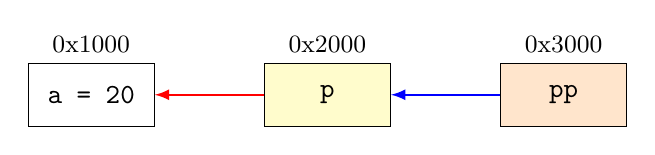
\begin{tikzpicture}[
    box/.style={draw, minimum width=1.6cm, minimum height=0.8cm, align=center, font=\ttfamily},
    arrow/.style={->, >=latex, thick},
    lbl/.style={font=\small}
]
    \node[box] (a) at (0,0) {a = 20};
    \node[box, fill=yellow!20] (p) at (3,0) {p};
    \node[box, fill=orange!20] (pp) at (6,0) {pp};
    \draw[arrow, red] (p.west) -- (a.east);
    \draw[arrow, blue] (pp.west) -- (p.east);
    \node[lbl, above] at (a.north) {0x1000};
    \node[lbl, above] at (p.north) {0x2000};
    \node[lbl, above] at (pp.north) {0x3000};
\end{tikzpicture}
\caption{二级指针链式指向关系}
\label{fig:double_pointer}
\end{figure}

\section{动态内存管理}

C语言通过标准库 \texttt{<stdlib.h>} 提供在堆（Heap）上动态分配内存的能力。

\begin{itemize}
    \item \textbf{\texttt{malloc(size\_t size)}}：在堆上分配指定字节数的内存，返回 \texttt{void*}，内容未初始化（垃圾值）。
    \item \textbf{\texttt{calloc(size\_t n, size\_t size)}}：分配 $n$ 个大小为 \texttt{size} 的连续内存块，并自动初始化为 0。
    \item \textbf{\texttt{realloc(void* ptr, size\_t size)}}：重新调整已分配内存的大小。若新大小更大，原有数据保留，新增部分未初始化。
    \item \textbf{\texttt{free(void* ptr)}}：释放已分配的内存，防止内存泄漏。
\end{itemize}

\begin{lstlisting}[caption={动态内存管理示例}]
#include <stdlib.h>

int *arr = (int*)malloc(10 * sizeof(int));
if (arr == NULL) {
    // 内存分配失败处理
    return -1;
}

// 使用 arr...
arr[0] = 42;

// 使用完毕后必须释放
free(arr);
arr = NULL; // 避免悬垂指针（Dangling Pointer）
\end{lstlisting}

\textbf{关键注意事项}：

\begin{itemize}
    \item 每次 \texttt{malloc} 必须配对一次 \texttt{free}，否则造成内存泄漏。
    \item \texttt{free} 之后的指针应立即置为 \texttt{NULL}，避免悬垂指针被误用。
    \item 不可对同一块内存 \texttt{free} 两次（Double Free），会导致未定义行为。
\end{itemize}

\section{函数指针与回调}

函数指针允许将函数作为参数传递，实现回调机制和多态行为。

\begin{lstlisting}[caption={函数指针示例}]
int add(int a, int b) { return a + b; }
int sub(int a, int b) { return a - b; }

// 声明函数指针
int (*func_ptr)(int, int);

func_ptr = add;
printf("%d\n", func_ptr(3, 4)); // 输出 7

func_ptr = sub;
printf("%d\n", func_ptr(3, 4)); // 输出 -1
\end{lstlisting}

\begin{lstlisting}[caption={回调函数示例}]
// 通用排序比较函数原型
typedef int (*CompareFunc)(const void*, const void*);

void mySort(int arr[], int n, CompareFunc cmp) {
    // 排序过程中调用 cmp 比较元素
    for (int i = 0; i < n - 1; i++) {
        for (int j = 0; j < n - i - 1; j++) {
            if (cmp(&arr[j], &arr[j+1]) > 0) {
                int tmp = arr[j];
                arr[j] = arr[j+1];
                arr[j+1] = tmp;
            }
        }
    }
}
\end{lstlisting}

\section{\texttt{const} 与指针的组合}

\texttt{const} 修饰指针时有三种经典组合方式，含义各不相同：

\begin{lstlisting}[caption={const 与指针的三种组合}]
int a = 10, b = 20;

// 1. 指针常量：指针本身不可变，但指向的值可变
int *const p1 = &a;
*p1 = 30;     // OK
// p1 = &b;   // Error: p1 是常量

// 2. 常量指针：指向的值不可变，但指针本身可变
const int *p2 = &a;
// *p2 = 30;  // Error: *p2 是常量
p2 = &b;      // OK

// 3. 指向常量的常量指针：两者均不可变
const int *const p3 = &a;
// *p3 = 30;  // Error
// p3 = &b;   // Error
\end{lstlisting}

\textbf{记忆口诀}：\texttt{const} 在 \texttt{*} 左侧 $\to$ 值不可变；\texttt{const} 在 \texttt{*} 右侧 $\to$ 指针不可变。

\section{复杂指针声明解析}

在 C 语言中，指针与数组、函数的组合会产生复杂的声明。理解它们的关键是**从变量名开始，按照优先级向外结合**。

\subsection{指针数组 vs 数组指针}

\begin{figure}[H]
\centering
\begin{minipage}{0.95\textwidth}
\begin{lstlisting}[caption={指针数组与数组指针}]
int *p1[10];   // 指针数组：数组，包含 10 个 int* 指针
int (*p2)[10]; // 数组指针：指针，指向一个包含 10 个 int 的数组

// 解析技巧：
// [] 优先级高于 *，所以 p1 先和 [] 结合，是数组。
// () 强制优先级，所以 p2 先和 * 结合，是指针。
\end{lstlisting}
\end{minipage}
\end{figure}

\subsection{函数指针数组}

\begin{figure}[H]
\centering
\begin{minipage}{0.95\textwidth}
\begin{lstlisting}[caption={函数指针数组示例}]
int add(int a, int b) { return a + b; }
int sub(int a, int b) { return a - b; }

// 声明一个包含 2 个函数指针的数组
int (*ops[2])(int, int) = {add, sub};

printf("%d\n", ops[0](3, 4)); // 输出 7
printf("%d\n", ops[1](3, 4)); // 输出 -1
\end{lstlisting}
\end{minipage}
\end{figure}

\section{实战：单链表的 C 语言实现}

作为指针和结构体的综合练习，以下实现了一个带头结点的单链表，包含插入、删除和遍历操作。这是衔接《数据结构》课程的经典案例。

\begin{figure}[H]
\centering
\begin{minipage}{0.95\textwidth}
\begin{lstlisting}[caption={单链表完整实现}]
#include <stdio.h>
#include <stdlib.h>

// 节点定义
typedef struct Node {
    int data;
    struct Node *next;
} Node;

// 初始化带头结点的链表
Node* initList() {
    Node *head = (Node*)malloc(sizeof(Node));
    head->next = NULL;
    return head;
}

// 头插法
void insertHead(Node *head, int val) {
    Node *newNode = (Node*)malloc(sizeof(Node));
    newNode->data = val;
    newNode->next = head->next;
    head->next = newNode;
}

// 删除第一个值为 val 的节点
void deleteVal(Node *head, int val) {
    Node *prev = head;
    Node *curr = head->next;
    while (curr) {
        if (curr->data == val) {
            prev->next = curr->next;
            free(curr);
            return;
        }
        prev = curr;
        curr = curr->next;
    }
}

// 遍历打印
void printList(Node *head) {
    Node *curr = head->next;
    while (curr) {
        printf("%d -> ", curr->data);
        curr = curr->next;
    }
    printf("NULL\n");
}

// 释放整个链表
void freeList(Node *head) {
    Node *curr = head;
    while (curr) {
        Node *tmp = curr;
        curr = curr->next;
        free(tmp);
    }
}
\end{lstlisting}
\end{minipage}
\end{figure}

\clearpage
\chapter{运算符与位运算}

\section{运算符分类}

C语言提供了丰富的运算符，主要分为以下六大类：

\subsection{算术运算符}

\texttt{+}, \texttt{-}, \texttt{*}, \texttt{/}, \texttt{\%}（取余）, \texttt{++}（自增）, \texttt{--}（自减）。

\subsection{关系运算符}

\texttt{==}, \texttt{!=}, \texttt{>}, \texttt{>=}, \texttt{<}, \texttt{<=}.

\subsection{逻辑运算符}

\texttt{\&\&}（与）, \texttt{||}（或）, \texttt{!}（非）。

\textbf{注：逻辑运算符的"短路求值"特性}：在逻辑表达式中，一旦前面的部分已经能够决定整个表达式的结果，编译器就会\textbf{停止执行}后面的表达式。

\begin{lstlisting}[caption={短路求值示例}]
int a = 0, b = 5;
// 因为 a == 0 为假，逻辑与 && 的最终结果注定为假，所以后面的 ++b 根本不会被执行！
if (a && (++b > 0)) { /* 不执行 */ }
printf("%d", b); // 输出仍为 5，而不是 6！
\end{lstlisting}

\subsection{位运算符}

\begin{itemize}
    \item \texttt{\&}（按位与）：有 0 则 0，全 1 才 1。
    \item \texttt{|}（按位或）：有 1 则 1，全 0 才 0。
    \item \texttt{\^{}}（按位异或）：不同为 1，相同为 0。
    \item \texttt{\textasciitilde}（按位取反）。
    \item \texttt{<<}（左移）、\texttt{>>}（右移）。
\end{itemize}

\textbf{移位运算的数学本质}：在不溢出的前提下，一个无符号整数\textbf{左移 n 位} \texttt{<< n} 相当于该数 $\times 2^n$；\textbf{右移 n 位} \texttt{>> n} 相当于该数 $\div 2^n$（向下取整）。这比直接用乘除法指令执行速度更快。

\subsection{赋值运算符}

\texttt{=}, \texttt{+=}, \texttt{-=} 等（包含存取/复合赋值）。

\subsection{杂项运算符}

\begin{itemize}
    \item \texttt{sizeof()}：返回类型或变量所占用的字节数（Byte）。
    \item \texttt{\&}：取地址符（获取变量的内存地址）。
    \item \texttt{*}：解引用符/间接寻址符（通过地址获取值）。
    \item \texttt{? :}：三目运算符（条件表达式，等价于 \texttt{if-else} 简写）。
    \item \texttt{()}, \texttt{[]}, \texttt{.}, \texttt{->}：括号、数组下标及结构体成员访问符。
\end{itemize}

\section{运算符优先级可视化}

从高到低的优先级顺序如下表所示。同一行内的运算符优先级相同，结合性决定求值方向。

\begin{figure}[H]
\centering
\begin{tikzpicture}[
    box/.style={draw, minimum width=11cm, minimum height=0.55cm, font=\ttfamily\small, align=left},
    lvl/.style={font=\bfseries\small, text=blue},
    arrow/.style={->, >=latex, thick}
]
    \node[lvl, anchor=east] (l1) at (-1.2, 0) {1 (最高)};
    \node[box] (b1) at (5, 0) {\texttt{()} \quad \texttt{[]} \quad \texttt{->} \quad \texttt{.}};
    
    \node[lvl, anchor=east] (l2) at (-1.2, -0.7) {2};
    \node[box] (b2) at (5, -0.7) {\texttt{++} \texttt{--} \texttt{!} \texttt{\textasciitilde} \texttt{sizeof} \texttt{\&} \texttt{*} \quad (单目/一元)};
    
    \node[lvl, anchor=east] (l3) at (-1.2, -1.4) {3};
    \node[box] (b3) at (5, -1.4) {\texttt{*} \texttt{/} \texttt{\%} \quad (乘、除、取余)};
    
    \node[lvl, anchor=east] (l4) at (-1.2, -2.1) {4};
    \node[box] (b4) at (5, -2.1) {\texttt{+} \texttt{-} \quad (加、减)};
    
    \node[lvl, anchor=east] (l5) at (-1.2, -2.8) {5};
    \node[box] (b5) at (5, -2.8) {\texttt{<<} \texttt{>>} \quad (移位)};
    
    \node[lvl, anchor=east] (l6) at (-1.2, -3.5) {6};
    \node[box] (b6) at (5, -3.5) {\texttt{<} \texttt{>} \texttt{<=} \texttt{>=} \quad (关系比较：大小)};
    
    \node[lvl, anchor=east] (l7) at (-1.2, -4.2) {7};
    \node[box] (b7) at (5, -4.2) {\texttt{==} \texttt{!=} \quad (关系比较：相等)};
    
    \node[lvl, anchor=east] (l8) at (-1.2, -4.9) {8};
    \node[box] (b8) at (5, -4.9) {\texttt{\&} \quad (按位与)};
    
    \node[lvl, anchor=east] (l9) at (-1.2, -5.6) {9};
    \node[box] (b9) at (5, -5.6) {\texttt{\^{}} \quad (按位异或)};
    
    \node[lvl, anchor=east] (l10) at (-1.2, -6.3) {10};
    \node[box] (b10) at (5, -6.3) {\texttt{|} \quad (按位或)};
    
    \node[lvl, anchor=east] (l11) at (-1.2, -7.0) {11};
    \node[box] (b11) at (5, -7.0) {\texttt{\&\&} \quad (逻辑与)};
    
    \node[lvl, anchor=east] (l12) at (-1.2, -7.7) {12};
    \node[box] (b12) at (5, -7.7) {\texttt{||} \quad (逻辑或)};
    
    \node[lvl, anchor=east] (l13) at (-1.2, -8.4) {13};
    \node[box] (b13) at (5, -8.4) {\texttt{?:} \quad (三目/条件)};
    
    \node[lvl, anchor=east] (l14) at (-1.2, -9.1) {14 (最低)};
    \node[box] (b14) at (5, -9.1) {\texttt{=} \texttt{+=} \texttt{-=} \dots \quad \texttt{,} \quad (赋值与逗号)};
    
    % 结合性标注
    \node[font=\small, anchor=west] at (11, 0) {$\leftarrow$ 左结合};
    \node[font=\small, anchor=west] at (11, -0.7) {$\leftarrow$ 右结合};
    \node[font=\small, anchor=west] at (11, -4.9) {$\leftarrow$ 左结合};
    \node[font=\small, anchor=west] at (11, -8.4) {$\leftarrow$ 右结合};
    \node[font=\small, anchor=west] at (11, -9.1) {$\leftarrow$ 右结合};
\end{tikzpicture}
\caption{C语言运算符优先级全图（从上到下优先级递减）}
\label{fig:operator_priority}
\end{figure}

\textbf{工程建议}：当表达式涉及多种运算符混合时，不要依赖记忆优先级，而是\textbf{显式使用括号}来明确意图。

\section{位运算高级技巧}

\subsection{异或（XOR）原地值交换算法（无需临时变量）}

利用 \texttt{A \textasciicircum{} B} 相同为0、不同为1以及自反的特性，可以不借助临时变量交换两个整数：

\begin{lstlisting}[caption={XOR 交换算法}]
// 假设 int a = 60 (0011 1100), b = 13 (0000 1101)
a = a ^ b; // 得到中间值 0011 0001
b = a ^ b; // 此时 b 变为了原 a 的值 (0011 1100)
a = a ^ b; // 此时 a 变为了原 b 的值 (0000 1101)
\end{lstlisting}

\subsection{判断一个数是否为 2 的幂次 ($2^k$)}

利用 \texttt{n \& (n - 1)} 能够完美消除二进制中最低位 1 的数学特性：

\begin{lstlisting}[caption={2 的幂次判定}]
// 若成立，说明 n 的二进制表示中仅含有一个 1，即它是 2 的整数次幂
if ((n > 0) && (n & (n - 1)) == 0) { /* 是 2 的幂次 */ }
\end{lstlisting}

\subsection{常用位运算操作}

\begin{itemize}
    \item \textbf{置位（Set Bit）}：\texttt{n |= (1 << k)}，将第 $k$ 位置为 1。
    \item \textbf{清零（Clear Bit）}：\texttt{n \&= \textasciitilde(1 << k)}，将第 $k$ 位置为 0。
    \item \textbf{取反位（Toggle Bit）}：\texttt{n \textasciicircum{}= (1 << k)}，翻转第 $k$ 位。
    \item \textbf{检测位（Test Bit）}：\texttt{(n >> k) \& 1}，获取第 $k$ 位的值。
\end{itemize}

\section{原码、反码与补码}

计算机内部一律使用\textbf{补码}来存储和计算整数：

\begin{itemize}
    \item \textbf{原码}：最高位为符号位（0表示正，1表示负），其余位表示数值绝对值。
    \item \textbf{反码}：正数的反码与原码相同；负数的反码为原码除符号位外，其余各位按位取反（0变1，1变0）。
    \item \textbf{补码}：正数的补码与原码相同；负数的补码为\textbf{反码 + 1}。
\end{itemize}

\begin{figure}[H]
\centering
\begin{tikzpicture}[
    box/.style={draw, minimum width=1.8cm, minimum height=0.6cm, font=\ttfamily\small, align=center},
    arrow/.style={->, >=latex, thick},
    lbl/.style={font=\small}
]
    \node[lbl, anchor=east] at (-2, 0.5) {+5};
    \node[box] (a1) at (0, 0.5) {0000 0101};
    \node[box] (a2) at (2.5, 0.5) {0000 0101};
    \node[box] (a3) at (5, 0.5) {0000 0101};
    \node[lbl] at (0, 1.1) {原码};
    \node[lbl] at (2.5, 1.1) {反码};
    \node[lbl] at (5, 1.1) {补码};
    
    \node[lbl, anchor=east] at (-2, -0.5) {-5};
    \node[box] (b1) at (0, -0.5) {1000 0101};
    \node[box] (b2) at (2.5, -0.5) {1111 1010};
    \node[box] (b3) at (5, -0.5) {1111 1011};
    
    \draw[arrow] (b1.east) -- node[lbl, above] {符号位外取反} (b2.west);
    \draw[arrow] (b2.east) -- node[lbl, above] {+1} (b3.west);
\end{tikzpicture}
\caption{原码、反码、补码转换关系（以 8 位为例）}
\label{fig:complement}
\end{figure}

\clearpage
\chapter{存储类别与内存模型}

\section{存储类别 (Storage Classes)}

\begin{itemize}
    \item \textbf{\texttt{auto}（自动）}：默认类别。变量进入作用域时创建，离开时自动销毁。
    \item \textbf{\texttt{register}（寄存器）}：建议编译器将变量放入 CPU 寄存器以极大提升读取速度。限制为一个字长（如 4字节），且\textbf{无法对寄存器变量使用 \texttt{\&} 取地址符}。
    \item \textbf{\texttt{static}（静态）}：具有隐藏和保持数据的作用。
    \item \textbf{\texttt{extern}（外部声明）}：用于告诉编译器，该变量或函数的定义在别的文件中。
\end{itemize}

\section{内存四区模型}

C程序运行时，操作系统将进程的虚拟地址空间划分为四个主要区域，每个区域承担不同的存储职责。

\begin{figure}[H]
\centering
\begin{tikzpicture}[
    zone/.style={draw, minimum width=5cm, minimum height=1.2cm, align=center, font=\small},
    arrow/.style={->, >=latex, thick},
    lbl/.style={font=\small}
]
    % 高地址
    \node[lbl, anchor=west] at (3.5, 3.0) {$\uparrow$ 高地址};
    
    % 代码区
    \node[zone, fill=green!15] (code) at (0, 2.2) {代码区 (Text)};
    \node[lbl, anchor=west] at (3, 2.2) {存放编译后的机器指令，只读};
    
    % 全局/静态区
    \node[zone, fill=yellow!20] (global) at (0, 0.8) {全局/静态区 (Data/BSS)};
    \node[lbl, anchor=west] at (3, 0.8) {全局变量、static 变量};
    
    % 堆区
    \node[zone, fill=orange!15] (heap) at (0, -0.6) {堆区 (Heap)};
    \node[lbl, anchor=west] at (3, -0.6) {malloc/calloc/realloc 动态分配};
    
    % 增长箭头
    \draw[arrow, blue, thick] (2.8, -0.2) -- node[lbl, right] {向上增长} (2.8, -1.2);
    
    % 栈区
    \node[zone, fill=red!15] (stack) at (0, -2.0) {栈区 (Stack)};
    \node[lbl, anchor=west] at (3, -2.0) {局部变量、函数调用帧};
    
    % 增长箭头
    \draw[arrow, blue, thick] (2.8, -1.6) -- node[lbl, right] {向下增长} (2.8, -2.6);
    
    % 低地址
    \node[lbl, anchor=west] at (3.5, -3.0) {$\downarrow$ 低地址};
\end{tikzpicture}
\caption{C程序运行时内存四区布局}
\label{fig:memory_zones}
\end{figure}

\begin{enumerate}
    \item \textbf{代码区 (Text Segment)}：存放编译后的机器指令。该区域在物理上被标记为只读，任何尝试修改代码区内容的操作都会触发段错误（Segmentation Fault）。
    \item \textbf{全局/静态区 (Data/BSS Segment)}：
    \begin{itemize}
        \item \textbf{Data 段}：存放已初始化的全局变量和静态变量。
        \item \textbf{BSS 段}：存放未初始化或初始化为 0 的全局变量和静态变量，程序加载时由系统自动清零。
    \end{itemize}
    \item \textbf{堆区 (Heap)}：由程序员通过 \texttt{malloc}、\texttt{calloc}、\texttt{realloc} 手动申请和 \texttt{free} 手动释放。堆区向高地址方向增长。若只申请不释放，将导致内存泄漏。
    \item \textbf{栈区 (Stack)}：由编译器自动管理。函数调用时在栈上压入栈帧（Stack Frame），包含局部变量、参数和返回地址。函数返回时栈帧自动弹出。栈区向低地址方向增长。栈空间有限（通常几 MB），递归过深会导致栈溢出。
\end{enumerate}

\section{\texorpdfstring{\texttt{static} 关键字的"双重人格"}{static 关键字的双重人格}}

\texttt{static} 在 C语言中修饰局部变量和修饰全局变量/函数时的作用完全不同：

\begin{enumerate}
    \item \textbf{修饰局部变量（延长生命周期）}：函数调用结束后，该变量不会被销毁，其值会保留供下一次调用使用。它被存储在静态存储区（而非栈区），只在初次运行时初始化一次。
    \item \textbf{修饰全局变量/函数（隐藏可见性）}：限制该全局变量或函数只能在当前 \texttt{.c} 文件内部被访问，其他文件即使使用 \texttt{extern} 也无法引用它，从而避免了跨文件命名的冲突。
\end{enumerate}

\begin{lstlisting}[caption={static 修饰局部变量}]
void counter() {
    static int count = 0;  // 仅首次调用时初始化为 0
    count++;
    printf("%d ", count);
}

int main() {
    counter(); // 输出 1
    counter(); // 输出 2
    counter(); // 输出 3
    return 0;
}
\end{lstlisting}

\section{类型导出定义 (typedef)}

\begin{itemize}
    \item \textbf{作用}：为已有数据类型定义一个新的易读别名。
\end{itemize}

\begin{lstlisting}[caption={typedef 使用示例}]
typedef unsigned char byte; // 将 unsigned char 取别名为 byte
byte b1, b2;               // 声明变量，等价于 unsigned char b1, b2;
\end{lstlisting}

\section{位域 (Bit Fields)}

允许在结构体中以"位（Bit）"为单位分配内存，常用于底层寄存器配置或网络协议解析：

\begin{lstlisting}[caption={位域示例}]
struct Register {
    unsigned int low_bit  : 1;  // 仅占 1 位
    unsigned int mid_bits : 3;  // 占用 3 位
};
\end{lstlisting}

\section{共用体 (Union)}

所有成员共享同一块内存，总大小等于其最大成员的大小。

\subsection{利用 \texttt{union} 检测系统大端序和小端序 (Endianness)}

大端序指高位字节存放在低地址，小端序指低位字节存放在低地址。我们可以用一段精简的共用体代码轻松检测当前计算机架构：

\begin{lstlisting}[caption={端序检测示例}]
#include <stdio.h>
union EndianCheck {
    int i;
    char c;
};

int main() {
    union EndianCheck ec;
    ec.i = 1; // 十六进制为 0x00000001
    
    // 如果 c == 1，说明低地址存储的是低位数据（0x01），为小端序（大部分现代 PC 架构）
    if (ec.c == 1) {
        printf("当前系统为：小端序 (Little Endian)\n");
    } else {
        printf("当前系统为：大端序 (Big Endian)\n");
    }
    return 0;
}
\end{lstlisting}

\begin{figure}[H]
\centering
\begin{tikzpicture}[
    box/.style={draw, minimum width=1.2cm, minimum height=0.6cm, font=\ttfamily\small, align=center},
    lbl/.style={font=\small},
    arrow/.style={->, >=latex, thick}
]
    % 小端序
    \node[lbl] at (0, 1.5) {小端序 (Little Endian)};
    \node[box] (le0) at (-2, 0.8) {0x01};
    \node[box] (le1) at (-0.7, 0.8) {0x00};
    \node[box] (le2) at (0.6, 0.8) {0x00};
    \node[box] (le3) at (1.9, 0.8) {0x00};
    \node[lbl] at (-2, 0.2) {低地址};
    \node[lbl] at (1.9, 0.2) {高地址};
    
    % 大端序
    \node[lbl] at (0, -0.8) {大端序 (Big Endian)};
    \node[box] (be0) at (-2, -1.5) {0x00};
    \node[box] (be1) at (-0.7, -1.5) {0x00};
    \node[box] (be2) at (0.6, -1.5) {0x00};
    \node[box] (be3) at (1.9, -1.5) {0x01};
    \node[lbl] at (-2, -2.1) {低地址};
    \node[lbl] at (1.9, -2.1) {高地址};
\end{tikzpicture}
\caption{大端序与小端序的内存字节排列对比}
\label{fig:endianness}
\end{figure}

\clearpage
\chapter{输入输出与文件}

\section{C语言输入输出核心概念}

\begin{itemize}
    \item \textbf{所有的设备都是文件（标准文件）}：\texttt{stdin}（键盘）、\texttt{stdout}（屏幕）、\texttt{stderr}（标准错误输出）。
    \item \textbf{封装形式}：以上文件及I/O函数都统一封装在标准库 \texttt{<stdio.h>} 中。
\end{itemize}

\section{\texorpdfstring{\texttt{stdio.h} 的函数管理}{stdio.h 的函数管理}}

\subsection{格式化输出：\texttt{printf}}

\begin{itemize}
    \item \textbf{原型}：\texttt{printf(const char* format, ...);}
    \item \textbf{作用}：格式化输出字符到屏幕。
\end{itemize}

\subsection{格式化输入：\texttt{scanf}}

\begin{itemize}
    \item \textbf{原型}：\texttt{scanf(const char* format, ...);}
    \item \textbf{作用}：从屏幕按某个格式获取一个值。
    \item \textbf{参数说明}：
    \begin{itemize}
        \item \texttt{format}：是一个格式字符串，用于指定输出/输入的格式。
        \item \texttt{...}：是一个可变长的参数列表，对应每一个前方的格式说明符的数据。
        \item \textbf{格式说明符}：如 \texttt{\%d}（整型）、\texttt{\%ld}（长整型）、\texttt{\%.3f} 等，代表这个占位的区域存放什么类型的数据。
        \item \textbf{转义字符}：一个既定的组合，表示一个特殊的意义。例如：\texttt{\textbackslash n}（换行）、\texttt{\textbackslash r}（回车）、\texttt{\textbackslash t}（制表符）、\texttt{\textbackslash b}（退格）。
    \end{itemize}
\end{itemize}

\subsection{字符级 I/O}

\begin{itemize}
    \item \textbf{\texttt{int getchar()}}：从屏幕读取下一个可用的字符（从当前字符集）。
    \item \textbf{\texttt{int putchar(int c)}}：输出到屏幕某一个字符（从当前字符集）。
\end{itemize}

\subsection{字符串级 I/O}

\begin{itemize}
    \item \textbf{\texttt{char* fgets(char* str, int n, FILE* stream);}}：从某个标准流中读取一些字符串。\texttt{n} 是从流中读取字符的个数。
    \item \textbf{\texttt{int fputs(const char* str, FILE* stream);}}：朝某个标准流注入字符串。\texttt{str} 是一个用于存放字符串的数组；\texttt{stream} 是一个标准流的指针。
\end{itemize}

\subsection{\texorpdfstring{现代 C语言中 \texttt{gets()} 的重大安全隐患}{gets() 的安全隐患}}

老课本常提到的 \texttt{gets(str)} 因为\textbf{无法限制读取输入的长度}，极易导致缓冲区溢出（Buffer Overflow）甚至导致系统崩溃或被黑客攻击。\textbf{在现代 C 标准（C11及以后）中已经被完全废弃}。

\textbf{标准替代方案}：请一律使用 \texttt{fgets} 代替。

\begin{lstlisting}[caption={安全的字符串读取}]
char buf[100];
// 最多只读取 99 个字符，并在末尾自动补 '\0'，绝对不会发生内存越界溢出
fgets(buf, sizeof(buf), stdin); 
\end{lstlisting}

\section{文件操作}

\subsection{打开与关闭文件}

\begin{itemize}
    \item \textbf{\texttt{FILE* fopen(const char* filename, const char* mode);}}：以流形式的某种模式打开文件。
    \begin{itemize}
        \item \texttt{filename}：是一个文件路径。
        \item \texttt{mode}：是一个访问模式符号，如 \texttt{r}/\texttt{w}/\texttt{a}（读/写/添），加上 \texttt{+} 表示拓展写模式。如果在后面追加 \texttt{"b"}（如 \texttt{"rb"}, \texttt{"wb"}）则代表以二进制流模式访问。
    \end{itemize}
    \item \textbf{\texttt{int fclose(FILE* fp);}}：关闭文件。正常关闭返回 \texttt{0}，发生错误返回 \texttt{EOF} (-1)。
\end{itemize}

\textbf{注：忘记 \texttt{fclose} 导致的资源泄漏}：每次 \texttt{fopen} 打开文件都会占用操作系统的文件描述符及内存缓冲区。如果写程序忘记执行 \texttt{fclose}，会导致系统资源耗尽。

\subsection{字符级文件 I/O}

\begin{itemize}
    \item \textbf{\texttt{int fputc(int c, FILE* fp);}}：向指定文件流中写入一个字符。
    \item \textbf{\texttt{int fgetc(FILE* fp);}}：从指定文件流中读取一个字符。
\end{itemize}

\section{二进制文件读写与块操作}

访问二进制文件时，访问模式必须添加一个 \texttt{b}，如 \texttt{rb} / \texttt{wb} / \texttt{ab} / \texttt{rb+} / \texttt{wb+} / \texttt{ab+}。

\begin{itemize}
    \item \textbf{\texttt{size\_t fread(void* ptr, size\_t size, size\_t count, FILE* stream);}}
    \item \textbf{\texttt{size\_t fwrite(const void* ptr, size\_t size, size\_t count, FILE* stream);}}
\end{itemize}

\subsection{特点与应用场景}

\begin{itemize}
    \item \textbf{特点}：1. 读写快；2. 无精度损失。
    \item \textbf{适用场景}：结构体、数组、图像、音频、视频。
    \item \textbf{高级特性}：具备一级加密的效果（由于非文本格式，无法直接通过常规文本编辑器直观查看，会显示为乱码）。
\end{itemize}

\section{完整文件操作示例}

\subsection{文本文件读写完整示例}

\begin{lstlisting}[caption={文本文件写入与读取}]
#include <stdio.h>

int main() {
    // 写入文件
    FILE *fp = fopen("data.txt", "w");
    if (fp == NULL) {
        printf("打开文件失败\n");
        return 1;
    }
    fprintf(fp, "姓名: %s\n", "张三");
    fprintf(fp, "成绩: %d\n", 95);
    fclose(fp);
    
    // 读取文件
    fp = fopen("data.txt", "r");
    if (fp == NULL) {
        printf("打开文件失败\n");
        return 1;
    }
    char buf[256];
    while (fgets(buf, sizeof(buf), fp) != NULL) {
        printf("%s", buf);
    }
    fclose(fp);
    return 0;
}
\end{lstlisting}

\subsection{二进制文件读写结构体完整示例}

\begin{lstlisting}[caption={二进制文件读写结构体数组}]
#include <stdio.h>

struct Student {
    char name[20];
    int age;
    float score;
};

int main() {
    struct Student students[3] = {
        {"Alice", 20, 95.5},
        {"Bob", 21, 88.0},
        {"Charlie", 19, 92.3}
    };
    
    // 写入二进制文件
    FILE *fp = fopen("students.dat", "wb");
    if (fp == NULL) return 1;
    fwrite(students, sizeof(struct Student), 3, fp);
    fclose(fp);
    
    // 读取二进制文件
    struct Student buffer[3];
    fp = fopen("students.dat", "rb");
    if (fp == NULL) return 1;
    fread(buffer, sizeof(struct Student), 3, fp);
    fclose(fp);
    
    for (int i = 0; i < 3; i++) {
        printf("姓名: %s, 年龄: %d, 成绩: %.1f\n",
               buffer[i].name, buffer[i].age, buffer[i].score);
    }
    return 0;
}
\end{lstlisting}

\subsection{文件位置指针操作}

\begin{itemize}
    \item \textbf{\texttt{long ftell(FILE* fp)}}：返回当前文件位置指针相对于文件开头的偏移量（字节数）。
    \item \textbf{\texttt{int fseek(FILE* fp, long offset, int whence)}}：将文件位置指针移动到指定位置。\texttt{whence} 可取 \texttt{SEEK\_SET}（文件开头）、\texttt{SEEK\_CUR}（当前位置）、\texttt{SEEK\_END}（文件末尾）。
    \item \textbf{\texttt{void rewind(FILE* fp)}}：将文件位置指针重置到文件开头，等价于 \texttt{fseek(fp, 0, SEEK\_SET)}。
\end{itemize}

\begin{lstlisting}[caption={fseek 随机访问示例}]
FILE *fp = fopen("data.bin", "rb");
// 跳过前 2 个结构体，直接读取第 3 个
fseek(fp, 2 * sizeof(struct Student), SEEK_SET);
struct Student third;
fread(&third, sizeof(struct Student), 1, fp);
fclose(fp);
\end{lstlisting}

\section{输入缓冲区陷阱与解决方案}

初学者最常遇到的 I/O Bug 是：在使用 \texttt{scanf} 读取数字后，紧接着使用 \texttt{fgets} 读取字符串，结果 \texttt{fgets} 直接跳过，读取到一个空行。

\subsection{问题根源}

\texttt{scanf} 在读取数字时，遇到非数字字符（如换行符 \texttt{\textbackslash n}）会停止读取，但会将该换行符留在输入缓冲区中。随后的 \texttt{fgets} 会立即读取到这个残留的换行符，认为已经读取了一行，从而跳过用户输入。

\begin{figure}[H]
\centering
\begin{minipage}{0.95\textwidth}
\begin{lstlisting}[caption={输入缓冲区陷阱演示}]
int age;
char name[50];

printf("请输入年龄: ");
scanf("%d", &age);  // 用户输入 "20<回车>"，scanf 读取 20，留下 \n

printf("请输入姓名: ");
fgets(name, sizeof(name), stdin); 
// fgets 立即读到残留的 \n，直接返回，导致 name 为空字符串！

printf("年龄: %d, 姓名: %s\n", age, name);
\end{lstlisting}
\end{minipage}
\end{figure}

\subsection{标准解决方案}

\begin{enumerate}
    \item \textbf{清空输入缓冲区}：在 \texttt{scanf} 后手动消耗掉残留字符，直到遇到换行符或 EOF。
    \item \textbf{统一使用 \texttt{fgets}}：放弃 \texttt{scanf}，全部使用 \texttt{fgets} 读取整行，再用 \texttt{sscanf} 或 \texttt{strtol} 解析。这是最安全、最推荐的做法。
\end{enumerate}

\begin{figure}[H]
\centering
\begin{minipage}{0.95\textwidth}
\begin{lstlisting}[caption={清空缓冲区与统一 fgets 方案}]
// 方法 1：手动清空缓冲区
int c;
while ((c = getchar()) != '\n' && c != EOF);

// 方法 2（推荐）：统一使用 fgets + sscanf
char buf[100];
int age;

printf("请输入年龄: ");
fgets(buf, sizeof(buf), stdin);
sscanf(buf, "%d", &age);  // 从缓冲区解析数字，安全且不会残留

printf("请输入姓名: ");
fgets(name, sizeof(name), stdin); // 正常等待用户输入
\end{lstlisting}
\end{minipage}
\end{figure}

\clearpage
\chapter{预处理器与工程实践}

\section{条件编译}

条件编译允许根据特定条件决定是否编译某段代码，是实现跨平台兼容和调试开关的核心工具。

\subsection{\texorpdfstring{\texttt{\#ifdef} / \texttt{\#ifndef} / \texttt{\#endif}}{\#ifdef / \#ifndef / \#endif}}

\begin{lstlisting}[caption={条件编译基本用法}]
#define DEBUG 1

#ifdef DEBUG
    printf("调试模式：变量 x = %d\n", x);
#endif

#ifndef MAX_SIZE
    #define MAX_SIZE 100
#endif
\end{lstlisting}

\begin{itemize}
    \item \texttt{\#ifdef MACRO}：如果 \texttt{MACRO} 已被 \texttt{\#define} 定义，则编译其后代码。
    \item \texttt{\#ifndef MACRO}：如果 \texttt{MACRO} 未被定义，则编译其后代码。
    \item \texttt{\#endif}：结束条件编译块。
    \item \texttt{\#else} / \texttt{\#elif}：可配合使用，形成多分支条件编译。
\end{itemize}

\subsection{\texorpdfstring{\texttt{\#if} 表达式编译}{\#if 表达式编译}}

\begin{lstlisting}[caption={if 表达式条件编译}]
#define VERSION 2

#if VERSION >= 3
    printf("版本 3 及以上功能\n");
#elif VERSION == 2
    printf("版本 2 功能\n");
#else
    printf("旧版本兼容代码\n");
#endif
\end{lstlisting}

\section{头文件保护符（Include Guard）}

在多文件项目中，同一头文件可能被多个源文件间接多次包含，导致重复声明错误。头文件保护符通过条件编译确保头文件内容仅被编译一次。

\subsection{传统 \texttt{\#ifndef} 保护模式}

\begin{lstlisting}[caption={头文件保护符}]
// student.h
#ifndef STUDENT_H
#define STUDENT_H

struct Student {
    char name[20];
    int age;
};

void printStudent(struct Student s);

#endif // STUDENT_H
\end{lstlisting}

命名约定：将头文件名转为大写，将点号替换为下划线，前后加下划线。例如 \texttt{my\_header.h} 转为 \texttt{MY\_HEADER\_H}。

\subsection{\texttt{\#pragma once} 模式}

\begin{lstlisting}[caption={pragma once}]
#pragma once

struct Student {
    char name[20];
    int age;
};
\end{lstlisting}

\texttt{\#pragma once} 是编译器扩展指令，现代编译器（GCC、Clang、MSVC）均支持。它由编译器在文件级别保证唯一包含，书写更简洁，但不属于 C 标准。在存在符号链接或同一文件多条路径的工程中，\texttt{\#ifndef} 模式更为可靠。

\section{多文件项目管理}

一个规范的 C 语言项目通常按以下结构组织：

\begin{figure}[H]
\centering
\begin{tikzpicture}[
    folder/.style={font=\ttfamily\small, align=left},
    arrow/.style={->, >=latex, thick},
    lbl/.style={font=\small}
]
    \node[folder, anchor=west] (root) at (0, 0) {project/};
    \node[folder, anchor=west] (inc) at (0.6, -0.6) {include/};
    \node[folder, anchor=west] (sh) at (1.4, -1.2) {student.h};
    \node[folder, anchor=west] (uh) at (1.4, -1.8) {utils.h};
    \node[folder, anchor=west] (src) at (0.6, -2.6) {src/};
    \node[folder, anchor=west] (mc) at (1.4, -3.2) {main.c};
    \node[folder, anchor=west] (sc) at (1.4, -3.8) {student.c};
    \node[folder, anchor=west] (uc) at (1.4, -4.4) {utils.c};
    \node[folder, anchor=west] (mk) at (0.6, -5.0) {Makefile};

    % 树形连线
    \draw[thick] (root.south west) ++(0.3,0) |- (inc.west);
    \draw[thick] (root.south west) ++(0.3,0) |- (src.west);
    \draw[thick] (root.south west) ++(0.3,0) |- (mk.west);
    \draw[thick] (inc.south west) ++(0.3,0) |- (sh.west);
    \draw[thick] (inc.south west) ++(0.3,0) |- (uh.west);
    \draw[thick] (src.south west) ++(0.3,0) |- (mc.west);
    \draw[thick] (src.south west) ++(0.3,0) |- (sc.west);
    \draw[thick] (src.south west) ++(0.3,0) |- (uc.west);

    % 注释
    \node[lbl, anchor=west, text=gray] at (3.2, -1.2) {结构体定义和函数声明};
    \node[lbl, anchor=west, text=gray] at (3.2, -1.8) {工具函数声明};
    \node[lbl, anchor=west, text=gray] at (3.2, -3.2) {主程序入口};
    \node[lbl, anchor=west, text=gray] at (3.2, -3.8) {student.h 的实现};
    \node[lbl, anchor=west, text=gray] at (3.2, -4.4) {utils.h 的实现};
    \node[lbl, anchor=west, text=gray] at (3.2, -5.0) {构建脚本};
\end{tikzpicture}
\caption{典型项目文件结构}
\label{fig:project_structure}
\end{figure}

\textbf{编译与链接流程}：

\begin{enumerate}
    \item 每个 \texttt{.c} 文件独立编译为 \texttt{.o} 目标文件。
    \item 链接器将所有 \texttt{.o} 文件和系统库合并为最终可执行文件。
    \item 修改某个 \texttt{.c} 文件时，只需重新编译该文件，无需重新编译整个项目。
\end{enumerate}

\section{Makefile 基础}

Makefile 是 Unix/Linux 系统下的自动化构建工具，用于管理多文件项目的编译流程。

\begin{lstlisting}[caption={简单 Makefile 示例}]
CC = gcc
CFLAGS = -Wall -Wextra -std=c11
TARGET = program
SRCS = src/main.c src/student.c src/utils.c
OBJS = $(SRCS:.c=.o)

$(TARGET): $(OBJS)
	$(CC) $(CFLAGS) -o $(TARGET) $(OBJS)

%.o: %.c
	$(CC) $(CFLAGS) -c $< -o $@

clean:
	rm -f $(OBJS) $(TARGET)
\end{lstlisting}

\begin{itemize}
    \item \texttt{CC}：指定编译器。
    \item \texttt{CFLAGS}：编译选项，\texttt{-Wall} 开启所有警告，\texttt{-Wextra} 开启额外警告，\texttt{-std=c11} 指定 C11 标准。
    \item \texttt{make}：执行构建。
    \item \texttt{make clean}：清理编译产物。
\end{itemize}

\section{常用编译选项}

\begin{table}[H]
\centering
\renewcommand{\arraystretch}{1.5}
\begin{tabulary}{\linewidth}{CCC}
\toprule
\textbf{选项} & \textbf{作用} \\ \midrule
\texttt{-Wall} & 开启所有常用警告 \\ 
\texttt{-Wextra} & 开启额外警告 \\ 
\texttt{-Werror} & 将警告视为错误，阻止编译通过 \\ 
\texttt{-g} & 生成调试信息（供 GDB 使用） \\ 
\texttt{-O0 / -O1 / -O2 / -O3} & 优化等级（0为不优化，3为最高优化） \\ 
\texttt{-std=c99 / c11 / c17} & 指定 C 语言标准版本 \\ 
\texttt{-o output} & 指定输出文件名 \\ 
\texttt{-c} & 仅编译不链接，生成 .o 文件 \\ 
\texttt{-I dir} & 添加头文件搜索路径 \\ 
\texttt{-l lib} & 链接指定库（如 \texttt{-lm} 链接数学库） \\ \bottomrule
\end{tabulary}
\caption{GCC 常用编译选项}
\label{tab:gcc_flags}
\end{table}

\section{调试技巧}

\subsection{使用 GDB 调试}

\begin{lstlisting}[caption={GDB 基本命令}]
gcc -g -o program main.c    // 编译时加 -g 生成调试信息
gdb ./program               // 启动 GDB

(gdb) break main            // 在 main 函数处设置断点
(gdb) run                   // 运行程序
(gdb) next                  // 单步执行（不进入函数）
(gdb) step                  // 单步执行（进入函数）
(gdb) print x               // 打印变量 x 的值
(gdb) continue              // 继续执行到下一个断点
(gdb) quit                  // 退出 GDB
\end{lstlisting}

\subsection{常见运行时错误排查}

\begin{itemize}
    \item \textbf{段错误 (Segmentation Fault)}：访问了非法内存地址，常见原因包括空指针解引用、数组越界、访问已释放的内存。
    \item \textbf{内存泄漏 (Memory Leak)}：\texttt{malloc} 分配的内存未调用 \texttt{free} 释放。可使用 Valgrind 工具检测。
    \item \textbf{未定义行为 (Undefined Behavior)}：如 signed integer overflow、use-after-free 等，编译器不保证任何结果，可能导致难以复现的随机 Bug。
\end{itemize}

\section{静态库与动态库}

在实际工程中，通常将常用的功能打包成库（Library），供多个项目复用。C 语言支持两种库：静态库和动态库。

\subsection{静态库 (Static Library)}

静态库在编译时直接将目标代码复制到最终的可执行文件中。生成的可执行文件体积较大，但运行时不需要额外的库文件。

\begin{figure}[H]
\centering
\begin{minipage}{0.95\textwidth}
\begin{lstlisting}[caption={静态库制作与使用 (Linux)}]
# 1. 编译目标文件
gcc -c math_utils.c -o math_utils.o

# 2. 打包为静态库 (libmath.a)
ar rcs libmath.a math_utils.o

# 3. 链接静态库
gcc main.c -L. -lmath -o program
# -L. 表示在当前目录查找库，-lmath 表示链接 libmath.a
\end{lstlisting}
\end{minipage}
\end{figure}

\subsection{动态库/共享库 (Shared Library)}

动态库在编译时仅记录引用信息，在程序运行时才加载到内存。多个程序可共享同一份动态库，节省内存和磁盘空间。

\begin{figure}[H]
\centering
\begin{minipage}{0.95\textwidth}
\begin{lstlisting}[caption={动态库制作与使用 (Linux)}]
# 1. 编译位置无关代码 (Position Independent Code)
gcc -c -fPIC math_utils.c -o math_utils.o

# 2. 打包为动态库 (libmath.so)
gcc -shared -o libmath.so math_utils.o

# 3. 链接动态库
gcc main.c -L. -lmath -o program

# 4. 运行时指定库路径（否则可能找不到 .so）
export LD_LIBRARY_PATH=.:$LD_LIBRARY_PATH
./program
\end{lstlisting}
\end{minipage}
\end{figure}

\section{从 Makefile 到 CMake}

Makefile 是 Unix/Linux 系统下的经典构建工具，但语法较为晦涩。现代 C/C++ 项目广泛采用 \textbf{CMake}，它通过跨平台的 \texttt{CMakeLists.txt} 脚本生成对应平台的构建系统（如 Makefile、Ninja、Visual Studio 工程）。

\begin{figure}[H]
\centering
\begin{minipage}{0.95\textwidth}
\begin{lstlisting}[caption={CMakeLists.txt 基础示例}]
cmake_minimum_required(VERSION 3.10)
project(MyProject C)

# 设置 C 标准
set(CMAKE_C_STANDARD 11)

# 添加可执行文件
add_executable(program src/main.c src/utils.c)

# 链接数学库
target_link_libraries(program m)
\end{lstlisting}
\end{minipage}
\end{figure}

\textbf{CMake 构建流程}：
\begin{enumerate}
    \item 在项目根目录创建 \texttt{CMakeLists.txt}。
    \item 运行 \texttt{cmake -S . -B build} 生成构建文件到 \texttt{build/} 目录。
    \item 运行 \texttt{cmake --build build} 执行编译。
\end{enumerate}

\section{未定义行为 (UB) 常见清单}

C 语言为了追求极致性能，将许多边界情况定义为"未定义行为"（Undefined Behavior, UB）。编译器不对 UB 做任何保证，可能导致程序崩溃、静默错误或看似正常但逻辑错误的结果。以下是最高频的 UB 清单：

\begin{table}[H]
\centering
\small
\renewcommand{\arraystretch}{1.5}
\begin{tabulary}{\linewidth}{CC}
\toprule
\textbf{未定义行为} & \textbf{示例代码} \\ \midrule
有符号整数溢出 & \texttt{int x = INT\_MAX; x++;} \\ 
解引用空指针 & \texttt{int *p = NULL; *p = 10;} \\ 
访问已释放内存 (Use-After-Free) & \texttt{free(p); *p = 5;} \\ 
数组越界访问 & \texttt{int a[5]; a[5] = 10;} \\ 
修改字符串字面量 & \texttt{char *s = "hello"; s[0] = 'H';} \\ 
同一表达式多次修改同一变量 & \texttt{int i = 0; i = i++;} \\ 
函数返回值类型不匹配 & 声明返回 \texttt{int} 但实际返回 \texttt{float} \\ \bottomrule
\end{tabulary}
\caption{C语言常见未定义行为 (UB) 清单}
\label{tab:ub_list}
\end{table}

\textbf{防御建议}：始终开启编译器警告（\texttt{-Wall -Wextra}），使用静态分析工具（如 Clang-Tidy、Cppcheck），并在关键逻辑中加入 \texttt{assert} 断言。

\clearpage
\appendix
\chapter{C标准库函数速查手册}

本章汇总 C语言标准库中最常用的函数，按头文件分类，提供函数原型、功能说明和简要示例。

\section{C标准库头文件总览}

\begin{table}[H]
\centering
\small
\renewcommand{\arraystretch}{1.5}
\begin{tabulary}{\linewidth}{CC}
\toprule
\textbf{头文件} & \textbf{主要功能} \\ \midrule
\texttt{<stdio.h>} & 标准输入输出、文件操作、格式化 I/O \\ 
\texttt{<stdlib.h>} & 内存管理、数值转换、随机数、程序控制、排序查找 \\ 
\texttt{<string.h>} & 字符串操作、内存操作 \\ 
\texttt{<math.h>} & 数学函数（三角、指数、对数、取整等） \\ 
\texttt{<ctype.h>} & 字符分类与大小写转换 \\ 
\texttt{<time.h>} & 时间与日期处理 \\ 
\texttt{<assert.h>} & 运行时断言调试 \\ 
\texttt{<errno.h>} & 错误码定义 \\ 
\texttt{<stdarg.h>} & 可变参数处理 \\ 
\texttt{<limits.h>} & 整型类型取值范围常量 \\ 
\texttt{<float.h>} & 浮点型精度与范围常量 \\ 
\texttt{<stddef.h>} & 常用类型定义（size\_t, ptrdiff\_t, NULL 等） \\ 
\texttt{<setjmp.h>} & 非局部跳转（setjmp/longjmp） \\ 
\texttt{<signal.h>} & 信号处理 \\ 
\texttt{<locale.h>} & 本地化设置 \\ 
\texttt{<stdbool.h>} & 布尔类型支持（C99） \\ 
\texttt{<inttypes.h>} & 固定宽度整型与格式化宏（C99） \\ \bottomrule
\end{tabulary}
\caption{C标准库头文件一览}
\label{tab:stdlib_overview}
\end{table}

\section{\texorpdfstring{\texttt{<stdio.h>} 标准输入输出库}{<stdio.h> 标准输入输出库}}

\subsection{格式化输入输出}

\begin{table}[H]
\centering
\renewcommand{\arraystretch}{1.6}
\begin{tabulary}{\linewidth}{CCC}
\toprule
\textbf{函数原型} & \textbf{功能说明} & \textbf{返回值} \\ \midrule
\texttt{int printf(const char* fmt, ...)} & 格式化输出到 stdout & 成功输出的字符数 \\ 
\texttt{int scanf(const char* fmt, ...)} & 从 stdin 格式化输入 & 成功赋值的参数个数 \\ 
\texttt{int fprintf(FILE* fp, const char* fmt, ...)} & 格式化输出到文件 & 成功输出的字符数 \\ 
\texttt{int fscanf(FILE* fp, const char* fmt, ...)} & 从文件格式化输入 & 成功赋值的参数个数 \\ 
\texttt{int sprintf(char* buf, const char* fmt, ...)} & 格式化输出到字符串缓冲区 & 写入的字符数（不含 \textbackslash 0） \\ 
\texttt{int snprintf(char* buf, size\_t n, const char* fmt, ...)} & 安全版 sprintf，限制最大写入 n 字节 & 应写入的字符数 \\ 
\texttt{int sscanf(const char* str, const char* fmt, ...)} & 从字符串格式化输入 & 成功赋值的参数个数 \\ \bottomrule
\end{tabulary}
\caption{stdio.h 格式化输入输出函数}
\label{tab:stdio_format}
\end{table}

\subsection{字符与字符串 I/O}

\begin{table}[H]
\centering
\small
\renewcommand{\arraystretch}{1.6}
\begin{tabulary}{\linewidth}{CCC}
\toprule
\textbf{函数原型} & \textbf{功能说明} & \textbf{返回值} \\ \midrule
\texttt{int getchar(void)} & 从 stdin 读取一个字符 & 读取的字符（EOF 表示结束） \\ 
\texttt{int putchar(int c)} & 向 stdout 输出一个字符 & 输出的字符（EOF 表示失败） \\ 
\texttt{int fgetc(FILE* fp)} & 从文件流读取一个字符 & 读取的字符（EOF 表示结束） \\ 
\texttt{int fputc(int c, FILE* fp)} & 向文件流写入一个字符 & 写入的字符（EOF 表示失败） \\ 
\texttt{char* fgets(char* s, int n, FILE* fp)} & 从文件流读取最多 n-1 个字符 & s 指针（NULL 表示失败/结束） \\ 
\texttt{int fputs(const char* s, FILE* fp)} & 向文件流写入字符串（不含 \textbackslash 0） & 非负值成功，EOF 失败 \\ 
\texttt{char* gets(char* s)} & \textbf{已废弃}：从 stdin 读取一行，无长度限制 & s 指针（\textbf{存在缓冲区溢出风险}） \\ \bottomrule
\end{tabulary}
\caption{stdio.h 字符与字符串 I/O 函数}
\label{tab:stdio_char}
\end{table}

\subsection{文件操作}

\begin{table}[H]
\centering
\small
\renewcommand{\arraystretch}{1.5}
\begin{tabulary}{\linewidth}{CCC}
\toprule
\textbf{函数原型} & \textbf{功能说明} & \textbf{返回值} \\ \midrule
\texttt{FILE* fopen(const char* path, const char* mode)} & 以指定模式打开文件 & FILE 指针（NULL 表示失败） \\ 
\texttt{int fclose(FILE* fp)} & 关闭文件并刷新缓冲区 & 0 成功，EOF 失败 \\ 
\texttt{size\_t fread(void* ptr, size\_t sz, size\_t n, FILE* fp)} & 从文件读取 n 个大小为 sz 的数据块 & 实际读取的块数 \\ 
\texttt{size\_t fwrite(const void* ptr, size\_t sz, size\_t n, FILE* fp)} & 向文件写入 n 个大小为 sz 的数据块 & 实际写入的块数 \\ 
\texttt{int fseek(FILE* fp, long off, int whence)} & 移动文件位置指针 & 0 成功，非零失败 \\ 
\texttt{long ftell(FILE* fp)} & 获取当前文件位置偏移量 & 偏移量（-1L 表示失败） \\ 
\texttt{void rewind(FILE* fp)} & 将文件位置指针重置到开头 & 无 \\ 
\texttt{int feof(FILE* fp)} & 检测是否到达文件末尾 & 非零表示已到末尾 \\ 
\texttt{int ferror(FILE* fp)} & 检测文件流是否发生错误 & 非零表示有错误 \\ 
\texttt{int remove(const char* path)} & 删除指定文件 & 0 成功，非零失败 \\ 
\texttt{int rename(const char* old, const char* new)} & 重命名文件 & 0 成功，非零失败 \\ 
\texttt{void clearerr(FILE* fp)} & 清除文件流的错误和 EOF 标志 & 无 \\ 
\texttt{void setbuf(FILE* fp, char* buf)} & 设置文件流的缓冲区 & 无 \\ 
\texttt{int fflush(FILE* fp)} & 刷新输出缓冲区，将数据写入文件 & 0 成功，EOF 失败 \\ \bottomrule
\end{tabulary}
\caption{stdio.h 文件操作函数}
\label{tab:stdio_file}
\end{table}

\subsection{其他 I/O 与错误处理}

\begin{table}[H]
\centering
\small
\renewcommand{\arraystretch}{1.5}
\begin{tabulary}{\linewidth}{CCC}
\toprule
\textbf{函数原型} & \textbf{功能说明} & \textbf{返回值} \\ \midrule
\texttt{int ungetc(int c, FILE* fp)} & 将字符 c 推回流中 & 推入的字符（EOF 表示失败） \\ 
\texttt{void perror(const char* msg)} & 将错误信息输出到 stderr & 格式为 \texttt{msg: strerror(errno)} \\ 
\texttt{int setvbuf(FILE* fp, char* buf, int mode, size\_t size)} & 设置流的缓冲模式与缓冲区 & 0 成功，非零失败 \\ 
\texttt{FILE* tmpfile(void)} & 创建临时二进制文件（关闭自动删除） & FILE 指针（NULL 表示失败） \\ 
\texttt{char* tmpnam(char* s)} & 生成唯一的临时文件名 & 指向文件名的指针 \\ \bottomrule
\end{tabulary}
\caption{stdio.h 其他 I/O 与错误处理函数}
\label{tab:stdio_other}
\end{table}

\section{\texorpdfstring{\texttt{<stdlib.h>} 标准通用工具库}{<stdlib.h> 标准通用工具库}}

\subsection{内存管理}

\begin{table}[H]
\centering
\small
\renewcommand{\arraystretch}{1.6}
\begin{tabulary}{\linewidth}{CCC}
\toprule
\textbf{函数原型} & \textbf{功能说明} & \textbf{返回值} \\ \midrule
\texttt{void* malloc(size\_t size)} & 分配 size 字节的未初始化内存 & 指向分配内存的指针（NULL 失败） \\ 
\texttt{void* calloc(size\_t n, size\_t sz)} & 分配 n*sz 字节并初始化为 0 & 指向分配内存的指针（NULL 失败） \\ 
\texttt{void* realloc(void* ptr, size\_t sz)} & 重新调整已分配内存的大小 & 新指针（NULL 失败，原内存不变） \\ 
\texttt{void free(void* ptr)} & 释放之前分配的内存 & 无 \\ \bottomrule
\end{tabulary}
\caption{stdlib.h 内存管理函数}
\label{tab:stdlib_mem}
\end{table}

\subsection{数值转换}

\begin{table}[H]
\centering
\small
\renewcommand{\arraystretch}{1.6}
\begin{tabulary}{\linewidth}{CCC}
\toprule
\textbf{函数原型} & \textbf{功能说明} & \textbf{返回值} \\ \midrule
\texttt{int atoi(const char* str)} & 字符串转 int & 转换后的整数值 \\ 
\texttt{long atol(const char* str)} & 字符串转 long & 转换后的长整数值 \\ 
\texttt{long long atoll(const char* str)} & 字符串转 long long & 转换后的 long long 值 \\ 
\texttt{double atof(const char* str)} & 字符串转 double & 转换后的浮点值 \\ 
\texttt{long strtol(const char* s, char** end, int base)} & 字符串转 long，支持指定进制 & 转换结果，end 指向首个无效字符 \\ 
\texttt{double strtod(const char* s, char** end)} & 字符串转 double & 转换结果，end 指向首个无效字符 \\ \bottomrule
\end{tabulary}
\caption{stdlib.h 数值转换函数}
\label{tab:stdlib_conv}
\end{table}

\subsection{随机数与程序控制}

\begin{table}[H]
\centering
\small
\renewcommand{\arraystretch}{1.6}
\begin{tabulary}{\linewidth}{CCC}
\toprule
\textbf{函数原型} & \textbf{功能说明} & \textbf{返回值} \\ \midrule
\texttt{int rand(void)} & 生成 $[0, \text{RAND\_MAX}]$ 范围内的伪随机数 & 随机整数值 \\ 
\texttt{void srand(unsigned int seed)} & 设置随机数种子 & 无 \\ 
\texttt{void exit(int status)} & 立即终止程序，刷新并关闭所有流 & 不返回 \\ 
\texttt{void abort(void)} & 异常终止程序，生成 SIGABRT 信号 & 不返回 \\ 
\texttt{int atexit(void (*func)(void))} & 注册程序正常终止时调用的函数 & 0 成功，非零失败 \\ 
\texttt{int system(const char* cmd)} & 执行系统命令 & 命令返回值 \\ \bottomrule
\end{tabulary}
\caption{stdlib.h 随机数与程序控制函数}
\label{tab:stdlib_ctrl}
\end{table}

\subsection{查找与排序}

\begin{table}[H]
\centering
\small
\renewcommand{\arraystretch}{1.6}
\begin{tabulary}{\linewidth}{CCC}
\toprule
\textbf{函数原型} & \textbf{功能说明} & \textbf{返回值} \\ \midrule
\texttt{void qsort(void* base, size\_t n, size\_t sz, int (*cmp)(const void*, const void*))} & 对数组进行快速排序 & 无（原地排序） \\ 
\texttt{void* bsearch(const void* key, const void* base, size\_t n, size\_t sz, int (*cmp)(const void*, const void*))} & 在已排序数组中二分查找 & 指向匹配元素的指针（NULL 未找到） \\ \bottomrule
\end{tabulary}
\caption{stdlib.h 查找与排序函数}
\label{tab:stdlib_search}
\end{table}

\subsection{绝对值与除法}

\begin{table}[H]
\centering
\small
\renewcommand{\arraystretch}{1.5}
\begin{tabulary}{\linewidth}{CCC}
\toprule
\textbf{函数原型} & \textbf{功能说明} & \textbf{返回值} \\ \midrule
\texttt{int abs(int n)} & 计算整数的绝对值 & 绝对值 \\ 
\texttt{long labs(long n)} & 计算 long 的绝对值 & 绝对值 \\ 
\texttt{long long llabs(long long n)} & 计算 long long 的绝对值 (C99) & 绝对值 \\ 
\texttt{div\_t div(int num, int den)} & 整数除法（返回商和余数） & \texttt{div\_t} 结构体 \{quot, rem\} \\ 
\texttt{ldiv\_t ldiv(long num, long den)} & long 整数除法 & \texttt{ldiv\_t} 结构体 \\ \bottomrule
\end{tabulary}
\caption{stdlib.h 绝对值与除法函数}
\label{tab:stdlib_math}
\end{table}

\subsection{多字节与宽字符转换}

\begin{table}[H]
\centering
\small
\renewcommand{\arraystretch}{1.5}
\begin{tabulary}{\linewidth}{CCC}
\toprule
\textbf{函数原型} & \textbf{功能说明} & \textbf{返回值} \\ \midrule
\texttt{int mblen(const char* s, size\_t n)} & 获取多字节字符的字节数 & 字节数（-1 表示无效） \\ 
\texttt{int mbtowc(wchar\_t* wc, const char* s, size\_t n)} & 多字节字符转宽字符 & 字节数 \\ 
\texttt{int wctomb(char* s, wchar\_t wc)} & 宽字符转多字节字符 & 字节数 \\ 
\texttt{size\_t mbstowcs(wchar\_t* dest, const char* src, size\_t n)} & 多字节字符串转宽字符串 & 转换的宽字符数 \\ 
\texttt{size\_t wcstombs(char* dest, const wchar\_t* src, size\_t n)} & 宽字符串转多字节字符串 & 转换的字节数 \\ \bottomrule
\end{tabulary}
\caption{stdlib.h 多字节与宽字符转换函数}
\label{tab:stdlib_mb}
\end{table}

\section{\texorpdfstring{\texttt{<string.h>} 字符串处理库}{<string.h> 字符串处理库}}

\subsection{字符串操作}

\begin{table}[H]
\centering
\small
\renewcommand{\arraystretch}{1.6}
\begin{tabulary}{\linewidth}{CCC}
\toprule
\textbf{函数原型} & \textbf{功能说明} & \textbf{返回值} \\ \midrule
\texttt{size\_t strlen(const char* s)} & 计算字符串长度（不含 \textbackslash 0） & 字符个数 \\ 
\texttt{char* strcpy(char* dst, const char* src)} & 复制字符串（含 \textbackslash 0） & dst 指针 \\ 
\texttt{char* strncpy(char* dst, const char* src, size\_t n)} & 最多复制 n 个字符 & dst 指针 \\ 
\texttt{char* strcat(char* dst, const char* src)} & 拼接字符串到 dst 末尾 & dst 指针 \\ 
\texttt{char* strncat(char* dst, const char* src, size\_t n)} & 最多拼接 n 个字符 & dst 指针 \\ 
\texttt{int strcmp(const char* s1, const char* s2)} & 字典序比较两个字符串 & $<0$ s1小，$=0$ 相等，$>0$ s1大 \\ 
\texttt{int strncmp(const char* s1, const char* s2, size\_t n)} & 最多比较前 n 个字符 & 同上 \\ 
\texttt{char* strchr(const char* s, int c)} & 查找字符 c 首次出现的位置 & 指向该位置的指针（NULL 未找到） \\ 
\texttt{char* strrchr(const char* s, int c)} & 查找字符 c 最后一次出现的位置 & 指向该位置的指针（NULL 未找到） \\ 
\texttt{char* strstr(const char* haystack, const char* needle)} & 查找子串首次出现的位置 & 指向子串起始位置的指针（NULL 未找到） \\ 
\texttt{char* strtok(char* str, const char* delim)} & 按分隔符拆分字符串（内部维护状态） & 下一个 token 指针（NULL 表示结束） \\ 
\texttt{char* strdup(const char* s)} & 复制字符串（内部调用 malloc） & 新分配的字符串指针 \\ \bottomrule
\end{tabulary}
\caption{string.h 字符串操作函数}
\label{tab:string_ops}
\end{table}

\subsection{内存操作}

\begin{table}[H]
\centering
\small
\renewcommand{\arraystretch}{1.6}
\begin{tabulary}{\linewidth}{CCC}
\toprule
\textbf{函数原型} & \textbf{功能说明} & \textbf{返回值} \\ \midrule
\texttt{void* memcpy(void* dst, const void* src, size\_t n)} & 复制 n 字节（\textbf{不可重叠}） & dst 指针 \\ 
\texttt{void* memmove(void* dst, const void* src, size\_t n)} & 复制 n 字节（\textbf{可安全重叠}） & dst 指针 \\ 
\texttt{void* memset(void* ptr, int val, size\_t n)} & 将前 n 字节设置为 val & ptr 指针 \\ 
\texttt{int memcmp(const void* s1, const void* s2, size\_t n)} & 比较前 n 个字节 & $<0, =0, >0$ \\ 
\texttt{void* memchr(const void* s, int c, size\_t n)} & 在前 n 字节中查找值 c & 指向该位置的指针（NULL 未找到） \\ \bottomrule
\end{tabulary}
\caption{string.h 内存操作函数}
\label{tab:string_mem}
\end{table}

\subsection{其他字符串操作}

\begin{table}[H]
\centering
\small
\renewcommand{\arraystretch}{1.5}
\begin{tabulary}{\linewidth}{CCC}
\toprule
\textbf{函数原型} & \textbf{功能说明} & \textbf{返回值} \\ \midrule
\texttt{char* strerror(int errnum)} & 获取错误码对应的错误描述字符串 & 指向错误信息的指针 \\ 
\texttt{size\_t strspn(const char* s, const char* accept)} & 计算 s 开头完全由 accept 中字符组成的长度 & 匹配的字符数 \\ 
\texttt{size\_t strcspn(const char* s, const char* reject)} & 计算 s 开头不包含 reject 中字符的长度 & 匹配的字符数 \\ 
\texttt{char* strpbrk(const char* s, const char* accept)} & 查找 s 中首次出现 accept 中任意字符的位置 & 指向该位置的指针（NULL 未找到） \\ 
\texttt{int strcoll(const char* s1, const char* s2)} & 根据当前 locale 比较字符串 & $<0, =0, >0$ \\ 
\texttt{size\_t strxfrm(char* dst, const char* src, size\_t n)} & 将字符串转换为 locale 相关的比较格式 & 转换后的长度 \\ \bottomrule
\end{tabulary}
\caption{string.h 其他字符串操作函数}
\label{tab:string_other}
\end{table}

\section{\texorpdfstring{\texttt{<math.h>} 数学函数库}{<math.h> 数学函数库}}

\subsection{常用数学函数}

\begin{table}[H]
\centering
\small
\renewcommand{\arraystretch}{1.6}
\begin{tabulary}{\linewidth}{CCC}
\toprule
\textbf{函数原型} & \textbf{功能说明} & \textbf{返回值} \\ \midrule
\texttt{double sqrt(double x)} & 平方根 $\sqrt{x}$ & 平方根值 \\ 
\texttt{double pow(double x, double y)} & 幂运算 $x^y$ & 幂值 \\ 
\texttt{double exp(double x)} & 自然指数 $e^x$ & 指数值 \\ 
\texttt{double log(double x)} & 自然对数 $\ln x$ & 对数值 \\ 
\texttt{double log10(double x)} & 常用对数 $\log_{10} x$ & 对数值 \\ 
\texttt{double fabs(double x)} & 绝对值 $|x|$ & 绝对值 \\ 
\texttt{double ceil(double x)} & 向上取整 $\lceil x \rceil$ & 不小于 x 的最小整数 \\ 
\texttt{double floor(double x)} & 向下取整 $\lfloor x \rfloor$ & 不大于 x 的最大整数 \\ 
\texttt{double round(double x)} & 四舍五入 & 最接近的整数 \\ 
\texttt{double fmod(double x, double y)} & 浮点取余 $x - n \cdot y$ & 余数 \\ \bottomrule
\end{tabulary}
\caption{math.h 常用数学函数}
\label{tab:math_funcs}
\end{table}

\subsection{三角函数}

\begin{table}[H]
\centering
\small
\renewcommand{\arraystretch}{1.6}
\begin{tabulary}{\linewidth}{CCC}
\toprule
\textbf{函数原型} & \textbf{功能说明} & \textbf{返回值} \\ \midrule
\texttt{double sin(double x)} & 正弦（x 为弧度） & $\sin x$ \\ 
\texttt{double cos(double x)} & 余弦（x 为弧度） & $\cos x$ \\ 
\texttt{double tan(double x)} & 正切（x 为弧度） & $\tan x$ \\ 
\texttt{double asin(double x)} & 反正弦，定义域 $[-1, 1]$ & 弧度值 $[-\pi/2, \pi/2]$ \\ 
\texttt{double acos(double x)} & 反余弦，定义域 $[-1, 1]$ & 弧度值 $[0, \pi]$ \\ 
\texttt{double atan(double x)} & 反正切 & 弧度值 $(-\pi/2, \pi/2)$ \\ 
\texttt{double atan2(double y, double x)} & 双参数反正切（判定象限） & 弧度值 $(-\pi, \pi]$ \\ \bottomrule
\end{tabulary}
\caption{math.h 三角函数}
\label{tab:math_trig}
\end{table}

\subsection{双曲函数}

\begin{table}[H]
\centering
\small
\renewcommand{\arraystretch}{1.5}
\begin{tabulary}{\linewidth}{CCC}
\toprule
\textbf{函数原型} & \textbf{功能说明} & \textbf{返回值} \\ \midrule
\texttt{double sinh(double x)} & 双曲正弦 $\frac{e^x - e^{-x}}{2}$ & 双曲正弦值 \\ 
\texttt{double cosh(double x)} & 双曲余弦 $\frac{e^x + e^{-x}}{2}$ & 双曲余弦值 \\ 
\texttt{double tanh(double x)} & 双曲正切 $\frac{\sinh x}{\cosh x}$ & 双曲正切值 \\ \bottomrule
\end{tabulary}
\caption{math.h 双曲函数}
\label{tab:math_hyper}
\end{table}

\subsection{其他数学函数}

\begin{table}[H]
\centering
\small
\renewcommand{\arraystretch}{1.5}
\begin{tabulary}{\linewidth}{CCC}
\toprule
\textbf{函数原型} & \textbf{功能说明} & \textbf{返回值} \\ \midrule
\texttt{double cbrt(double x)} & 立方根 $\sqrt[3]{x}$ (C99) & 立方根值 \\ 
\texttt{double hypot(double x, double y)} & 计算 $\sqrt{x^2 + y^2}$（避免溢出） & 斜边长度 \\ 
\texttt{double log2(double x)} & 以 2 为底的对数 (C99) & 对数值 \\ 
\texttt{double trunc(double x)} & 截断小数部分 (C99) & 整数部分 \\ 
\texttt{double fmax(double x, double y)} & 返回两数中的较大值 (C99) & 较大值 \\ 
\texttt{double fmin(double x, double y)} & 返回两数中的较小值 (C99) & 较小值 \\ 
\texttt{int isnan(double x)} & 判断是否为 NaN (C99) & 非零为真，零为假 \\ 
\texttt{int isinf(double x)} & 判断是否为无穷大 (C99) & 非零为真，零为假 \\ 
\texttt{int isfinite(double x)} & 判断是否为有限值 (C99) & 非零为真，零为假 \\ \bottomrule
\end{tabulary}
\caption{math.h 其他数学函数}
\label{tab:math_other}
\end{table}

\vspace{0.5em}
\noindent\textbf{常量}：\texttt{M\_PI}（$\pi \approx 3.14159$）、\texttt{M\_E}（$e \approx 2.71828$）。编译时需链接数学库：\texttt{gcc -lm}。

\section{\texorpdfstring{\texttt{<ctype.h>} 字符分类与转换库}{<ctype.h> 字符分类与转换库}}

\begin{table}[H]
\centering
\renewcommand{\arraystretch}{1.6}
\begin{tabulary}{\linewidth}{CCC}
\toprule
\textbf{函数原型} & \textbf{功能说明} & \textbf{返回值} \\ \midrule
\texttt{int isalpha(int c)} & 是否为字母（A-Z, a-z） & 非零为真，零为假 \\ 
\texttt{int isdigit(int c)} & 是否为数字（0-9） & 非零为真，零为假 \\ 
\texttt{int isalnum(int c)} & 是否为字母或数字 & 非零为真，零为假 \\ 
\texttt{int isspace(int c)} & 是否为空白字符（空格、\textbackslash t、\textbackslash n 等） & 非零为真，零为假 \\ 
\texttt{int isupper(int c)} & 是否为大写字母 & 非零为真，零为假 \\ 
\texttt{int islower(int c)} & 是否为小写字母 & 非零为真，零为假 \\ 
\texttt{int ispunct(int c)} & 是否为标点符号 & 非零为真，零为假 \\ 
\texttt{int iscntrl(int c)} & 是否为控制字符 & 非零为真，零为假 \\ 
\texttt{int isgraph(int c)} & 是否为图形字符（除空格外的可打印字符） & 非零为真，零为假 \\ 
\texttt{int isxdigit(int c)} & 是否为十六进制数字（0-9, a-f, A-F） & 非零为真，零为假 \\ 
\texttt{int isblank(int c)} & 是否为空白字符（空格或制表符，C99） & 非零为真，零为假 \\ 
\texttt{int isprint(int c)} & 是否为可打印字符 & 非零为真，零为假 \\ 
\texttt{int toupper(int c)} & 转为大写 & 大写字符 \\ 
\texttt{int tolower(int c)} & 转为小写 & 小写字符 \\ \bottomrule
\end{tabulary}
\caption{ctype.h 字符分类与转换函数}
\label{tab:ctype_funcs}
\end{table}

\section{\texorpdfstring{\texttt{<time.h>} 时间与日期库}{<time.h> 时间与日期库}}

\begin{table}[H]
\centering
\renewcommand{\arraystretch}{1.6}
\begin{tabulary}{\linewidth}{CCC}
\toprule
\textbf{函数原型} & \textbf{功能说明} & \textbf{返回值} \\ \midrule
\texttt{time\_t time(time\_t* t)} & 获取当前日历时间（秒数） & 从 1970-01-01 起的秒数 \\ 
\texttt{double difftime(time\_t t2, time\_t t1)} & 计算两个时间之差 & 秒数差值 \\ 
\texttt{struct tm* localtime(const time\_t* t)} & 将时间戳转为本地时间结构体 & tm 结构体指针 \\ 
\texttt{struct tm* gmtime(const time\_t* t)} & 将时间戳转为 UTC 时间结构体 & tm 结构体指针 \\ 
\texttt{time\_t mktime(struct tm* tm)} & 将 tm 结构体转为时间戳 & time\_t 值 \\ 
\texttt{char* asctime(const struct tm* tm)} & 将 tm 结构体转为可读字符串 & 字符串指针 \\ 
\texttt{char* ctime(const time\_t* t)} & 将时间戳转为可读字符串 & 字符串指针 \\ 
\texttt{size\_t strftime(char* s, size\_t max, const char* fmt, const struct tm* tm)} & 按格式将 tm 转为字符串 & 写入的字符数 \\ 
\texttt{clock\_t clock(void)} & 获取程序运行至今的 CPU 时间 & clock\_t 值（除以 CLOCKS\_PER\_SEC 得秒） \\ \bottomrule
\end{tabulary}
\caption{time.h 时间与日期函数}
\label{tab:time_funcs}
\end{table}

\noindent\begin{minipage}{\textwidth}
\begin{lstlisting}[caption={time.h 使用示例}]
#include <stdio.h>
#include <time.h>

int main() {
    time_t now = time(NULL);
    struct tm* local = localtime(&now);
    printf("当前时间: %d-%02d-%02d %02d:%02d:%02d\n",
           local->tm_year + 1900, local->tm_mon + 1, local->tm_mday,
           local->tm_hour, local->tm_min, local->tm_sec);
    return 0;
}
\end{lstlisting}
\end{minipage}

\vspace{0.5em}
\begin{sloppypar}
\noindent\textbf{结构体说明}：\texttt{struct timespec} 包含 \texttt{tv\_sec}（秒数）和 \texttt{tv\_nsec}（纳秒数），用于高精度时间表示（POSIX/C11）。
\end{sloppypar}

\section{\texorpdfstring{\texttt{<assert.h>} 断言库}{<assert.h> 断言库}}

\begin{table}[H]
\centering
\renewcommand{\arraystretch}{1.6}
\begin{tabulary}{\linewidth}{CCC}
\toprule
\textbf{宏/函数} & \textbf{功能说明} & \textbf{行为} \\ \midrule
\texttt{assert(expression)} & 运行时断言检查 & 表达式为假时打印错误信息并调用 abort() \\ 
\texttt{NDEBUG} & 宏定义 & 在 \texttt{\#include <assert.h>} 前定义 \texttt{NDEBUG} 可禁用所有 assert \\ \bottomrule
\end{tabulary}
\caption{assert.h 断言宏}
\label{tab:assert_funcs}
\end{table}

\noindent\begin{minipage}{\textwidth}
\begin{lstlisting}[caption={assert 使用示例}]
#include <assert.h>

int divide(int a, int b) {
    assert(b != 0);  // 如果 b 为 0，程序终止并输出错误信息
    return a / b;
}
\end{lstlisting}
\end{minipage}

\section{\texorpdfstring{\texttt{<errno.h>} 错误码库}{<errno.h> 错误码库}}

\begin{table}[H]
\centering
\renewcommand{\arraystretch}{1.6}
\begin{tabulary}{\linewidth}{CCC}
\toprule
\textbf{宏/变量} & \textbf{功能说明} & \textbf{典型值} \\ \midrule
\texttt{errno} & 全局错误码变量 & 由库函数在出错时设置 \\ 
\texttt{EDOM} & 数学函数定义域错误 & 如 sqrt(-1) \\ 
\texttt{ERANGE} & 结果超出表示范围 & 如溢出 \\ 
\texttt{EAGAIN} & 资源暂时不可用 & 非阻塞 I/O 场景 \\ 
\texttt{EINVAL} & 无效参数 & 传入非法参数 \\ \bottomrule
\end{tabulary}
\caption{errno.h 错误码}
\label{tab:errno_funcs}
\end{table}

\noindent\begin{minipage}{\textwidth}
\begin{lstlisting}[caption={errno 使用示例}]
#include <stdio.h>
#include <errno.h>
#include <string.h>
#include <math.h>

int main() {
    errno = 0;
    double result = sqrt(-1.0);
    if (errno == EDOM) {
        printf("数学定义域错误: %s\n", strerror(errno));
    }
    return 0;
}
\end{lstlisting}
\end{minipage}

\section{\texorpdfstring{\texttt{<stdarg.h>} 可变参数库}{<stdarg.h> 可变参数库}}

\begin{table}[H]
\centering
\renewcommand{\arraystretch}{1.6}
\begin{tabulary}{\linewidth}{CCC}
\toprule
\textbf{宏/类型} & \textbf{功能说明} & \textbf{用法} \\ \midrule
\texttt{va\_list} & 可变参数列表类型 & 用于声明参数遍历变量 \\ 
\texttt{va\_start(ap, last)} & 初始化 va\_list & last 是最后一个固定参数名 \\ 
\texttt{va\_arg(ap, type)} & 获取下一个参数 & type 为期望的参数类型 \\ 
\texttt{va\_end(ap)} & 清理 va\_list & 在函数返回前调用 \\ \bottomrule
\end{tabulary}
\caption{stdarg.h 可变参数宏}
\label{tab:stdarg_funcs}
\end{table}

\noindent\begin{minipage}{\textwidth}
\begin{lstlisting}[caption={可变参数函数示例}]
#include <stdio.h>
#include <stdarg.h>

double average(int count, ...) {
    va_list args;
    va_start(args, count);
    double sum = 0.0;
    for (int i = 0; i < count; i++) {
        sum += va_arg(args, double);
    }
    va_end(args);
    return sum / count;
}

int main() {
    printf("平均值: %.2f\n", average(4, 10.0, 20.0, 30.0, 40.0));
    return 0;
}
\end{lstlisting}
\end{minipage}

\section{\texorpdfstring{\texttt{<limits.h>} 与 \texttt{<float.h>} 极限值常量}{<limits.h> 与 <float.h> 极限值常量}}

\subsection{limits.h 整型极限}

\begin{table}[H]
\centering
\renewcommand{\arraystretch}{1.5}
\begin{tabulary}{\linewidth}{CCC}
\toprule
\textbf{宏} & \textbf{含义} & \textbf{典型值} \\ \midrule
\texttt{CHAR\_BIT} & char 的位数 & 8 \\ 
\texttt{CHAR\_MIN / CHAR\_MAX} & char 最小/最大值 & -128 / 127 \\ 
\texttt{INT\_MIN / INT\_MAX} & int 最小/最大值 & -2147483648 / 2147483647 \\ 
\texttt{LONG\_MIN / LONG\_MAX} & long 最小/最大值 & 平台相关 \\ 
\texttt{LLONG\_MIN / LLONG\_MAX} & long long 最小/最大值 & $\approx \pm 9.22 \times 10^{18}$ \\ 
\texttt{UINT\_MAX} & unsigned int 最大值 & 4294967295 \\ \bottomrule
\end{tabulary}
\caption{limits.h 常用宏常量}
\label{tab:limits_consts}
\end{table}

\subsection{float.h 浮点型极限}

\begin{table}[H]
\centering
\renewcommand{\arraystretch}{1.5}
\begin{tabulary}{\linewidth}{CCC}
\toprule
\textbf{宏} & \textbf{含义} & \textbf{典型值} \\ \midrule
\texttt{FLT\_MIN / DBL\_MIN} & float/double 最小正值 & $1.175 \times 10^{-38}$ / $2.225 \times 10^{-308}$ \\ 
\texttt{FLT\_MAX / DBL\_MAX} & float/double 最大值 & $3.402 \times 10^{38}$ / $1.797 \times 10^{308}$ \\ 
\texttt{FLT\_EPSILON / DBL\_EPSILON} & 机器精度 $\epsilon$ & $1.192 \times 10^{-7}$ / $2.220 \times 10^{-16}$ \\ 
\texttt{FLT\_DIG / DBL\_DIG} & 有效十进制位数 & 6 / 15 \\ \bottomrule
\end{tabulary}
\caption{float.h 常用宏常量}
\label{tab:float_consts}
\end{table}

\section{\texorpdfstring{\texttt{<stddef.h>} 标准定义库}{<stddef.h> 标准定义库}}

\begin{table}[H]
\centering
\small
\renewcommand{\arraystretch}{1.5}
\begin{tabulary}{\linewidth}{CCC}
\toprule
\textbf{宏/类型} & \textbf{说明} & \textbf{典型值/用法} \\ \midrule
\texttt{size\_t} & 无符号整型，用于表示对象大小 & \texttt{sizeof} 的返回类型 \\ 
\texttt{ptrdiff\_t} & 有符号整型，用于表示指针差值 & 两个指针相减的结果类型 \\ 
\texttt{wchar\_t} & 宽字符类型，用于存储宽字符 & 通常为 2 或 4 字节 \\ 
\texttt{NULL} & 空指针常量 & 通常定义为 \texttt{((void*)0)} 或 \texttt{0} \\ 
\texttt{offsetof(type, member)} & 计算结构体成员相对于起始地址的偏移量 & \texttt{offsetof(struct S, a)} \\ \bottomrule
\end{tabulary}
\caption{stddef.h 标准定义}
\label{tab:stddef}
\end{table}

\section{\texorpdfstring{\texttt{<setjmp.h>} 非局部跳转库}{<setjmp.h> 非局部跳转库}}

\begin{table}[H]
\centering
\small
\renewcommand{\arraystretch}{1.5}
\begin{tabulary}{\linewidth}{CCC}
\toprule
\textbf{宏/类型} & \textbf{功能说明} & \textbf{返回值/行为} \\ \midrule
\texttt{jmp\_buf} & 数组类型，用于保存调用环境（寄存器状态、栈指针等） & 供 \texttt{setjmp} 和 \texttt{longjmp} 使用 \\ 
\texttt{int setjmp(jmp\_buf env)} & 保存当前执行环境到 \texttt{env} 中 & 直接调用返回 0；通过 \texttt{longjmp} 返回非零值 \\ 
\texttt{void longjmp(jmp\_buf env, int val)} & 恢复到 \texttt{env} 保存的环境，并继续从 \texttt{setjmp} 处执行 & \texttt{setjmp} 将返回 \texttt{val}（若 val 为 0 则返回 1） \\ \bottomrule
\end{tabulary}
\caption{setjmp.h 非局部跳转宏}
\label{tab:setjmp}
\end{table}

\section{\texorpdfstring{\texttt{<signal.h>} 信号处理库}{<signal.h> 信号处理库}}

\begin{table}[H]
\centering
\small
\renewcommand{\arraystretch}{1.5}
\begin{tabulary}{\linewidth}{CCC}
\toprule
\textbf{宏/函数} & \textbf{功能说明} & \textbf{典型值/行为} \\ \midrule
\texttt{SIGINT} & 交互式注意信号（通常由 Ctrl+C 触发） & 值为 2 \\ 
\texttt{SIGTERM} & 终止请求信号 & 值为 15 \\ 
\texttt{SIGSEGV} & 无效内存访问（段错误） & 值为 11 \\ 
\texttt{SIG\_DFL} & 默认信号处理动作 & 恢复系统默认行为 \\ 
\texttt{SIG\_IGN} & 忽略信号 & 信号被丢弃，不执行任何操作 \\ 
\texttt{signal(int sig, void (*func)(int))} & 注册信号处理函数 & 返回旧的处理函数指针 \\ 
\texttt{raise(int sig)} & 向当前进程发送指定信号 & 成功返回 0，失败返回非零 \\ \bottomrule
\end{tabulary}
\caption{signal.h 信号处理宏与函数}
\label{tab:signal}
\end{table}

\section{\texorpdfstring{\texttt{<locale.h>} 本地化设置库}{<locale.h> 本地化设置库}}

\begin{table}[H]
\centering
\small
\renewcommand{\arraystretch}{1.5}
\begin{tabulary}{\linewidth}{CCC}
\toprule
\textbf{宏/函数} & \textbf{功能说明} & \textbf{典型值/行为} \\ \midrule
\texttt{LC\_ALL} & 设置所有本地化类别 & 涵盖数字、货币、时间、字符等 \\ 
\texttt{LC\_COLLATE} & 影响字符串比较和排序规则 & 如 \texttt{strcoll} 的行为 \\ 
\texttt{LC\_CTYPE} & 影响字符分类与转换函数 & 如 \texttt{isalpha}, \texttt{toupper} \\ 
\texttt{LC\_MONETARY} & 影响货币格式化 & 如 \texttt{localeconv} 返回的货币符号 \\ 
\texttt{LC\_NUMERIC} & 影响数字格式化（如小数点符号） & 如 \texttt{printf} 的小数点 \\ 
\texttt{LC\_TIME} & 影响日期和时间格式化 & 如 \texttt{strftime} 的输出 \\ 
\texttt{char* setlocale(int category, const char* locale)} & 设置或查询当前程序的本地化环境 & \texttt{""} 表示使用系统环境变量 \\ 
\texttt{struct lconv* localeconv(void)} & 获取当前本地化环境的数字和货币格式信息 & 返回指向 \texttt{lconv} 结构体的指针 \\ \bottomrule
\end{tabulary}
\caption{locale.h 本地化设置宏与函数}
\label{tab:locale}
\end{table}

\section{\texorpdfstring{\texttt{<stdbool.h>} 布尔类型库 (C99)}{<stdbool.h> 布尔类型库 (C99)}}

\begin{table}[H]
\centering
\small
\renewcommand{\arraystretch}{1.5}
\begin{tabulary}{\linewidth}{CC}
\toprule
\textbf{宏/类型} & \textbf{说明} \\ \midrule
\texttt{bool} & 扩展为 \texttt{\_Bool} 类型 \\ 
\texttt{true} & 扩展为整数常量 1 \\ 
\texttt{false} & 扩展为整数常量 0 \\ 
\texttt{\_\_bool\_true\_false\_are\_defined} & 扩展为 1，表示宏已定义 \\ \bottomrule
\end{tabulary}
\caption{stdbool.h 布尔类型宏}
\label{tab:stdbool}
\end{table}

\section{\texorpdfstring{\texttt{<inttypes.h>} 固定宽度整型库 (C99)}{<inttypes.h> 固定宽度整型库 (C99)}}

\begin{table}[H]
\centering
\small
\renewcommand{\arraystretch}{1.5}
\begin{tabulary}{\linewidth}{CCC}
\toprule
\textbf{类型/宏} & \textbf{说明} & \textbf{典型值} \\ \midrule
\texttt{int8\_t / uint8\_t} & 精确 8 位有符号/无符号整数 & 范围 $\pm 127$ / $0 \sim 255$ \\ 
\texttt{int16\_t / uint16\_t} & 精确 16 位有符号/无符号整数 & 范围 $\pm 32767$ / $0 \sim 65535$ \\ 
\texttt{int32\_t / uint32\_t} & 精确 32 位有符号/无符号整数 & 范围 $\pm 2\times 10^9$ / $0 \sim 4\times 10^9$ \\ 
\texttt{int64\_t / uint64\_t} & 精确 64 位有符号/无符号整数 & 范围 $\pm 9\times 10^{18}$ \\ 
\texttt{PRIu32 / PRId64} & \texttt{printf} 格式化固定宽度整型的宏 & 如 \texttt{PRIu32} 展开为 \texttt{"u"} \\ 
\texttt{SCNd32 / SCNu64} & \texttt{scanf} 格式化固定宽度整型的宏 & 如 \texttt{SCNd32} 展开为 \texttt{"d"} \\ \bottomrule
\end{tabulary}
\caption{inttypes.h 固定宽度整型与格式化宏}
\label{tab:inttypes}
\end{table}

\section{\texorpdfstring{\texttt{<tgmath.h>} 泛型数学宏库 (C99)}{<tgmath.h> 泛型数学宏库 (C99)}}

\begin{table}[H]
\centering
\small
\renewcommand{\arraystretch}{1.5}
\begin{tabulary}{\linewidth}{CCC}
\toprule
\textbf{泛型宏} & \textbf{功能说明} & \textbf{行为} \\ \midrule
\texttt{sin(x), cos(x), tan(x)} & 根据参数类型自动选择 float/double/long double 版本 & 传入 float 调用 \texttt{sinf}，传入 double 调用 \texttt{sin} \\ 
\texttt{sqrt(x), pow(x, y)} & 自动匹配数学函数变体 & 避免手动类型转换 \\ 
\texttt{fabs(x), ceil(x), floor(x)} & 自动选择绝对值、取整函数 & 支持整型与浮点型参数 \\ 
\texttt{atan2(y, x), hypot(x, y)} & 自动选择双参数函数版本 & 参数类型不同时提升为精度更高者 \\ \bottomrule
\end{tabulary}
\caption{tgmath.h 泛型数学宏}
\label{tab:tgmath}
\end{table}

\section{\texorpdfstring{\texttt{<wchar.h>} 宽字符 I/O 库 (C95)}{<wchar.h> 宽字符 I/O 库 (C95)}}

\begin{table}[H]
\centering
\small
\renewcommand{\arraystretch}{1.5}
\begin{tabulary}{\linewidth}{CCC}
\toprule
\textbf{函数原型} & \textbf{功能说明} & \textbf{返回值} \\ \midrule
\texttt{wint\_t fgetwc(FILE* fp)} & 从文件流读取一个宽字符 & 读取的宽字符（WEOF 表示结束） \\ 
\texttt{wint\_t fputwc(wchar\_t wc, FILE* fp)} & 向文件流写入一个宽字符 & 写入的宽字符（WEOF 表示失败） \\ 
\texttt{wchar\_t* fgetws(wchar\_t* s, int n, FILE* fp)} & 从文件流读取宽字符串 & s 指针（NULL 表示失败） \\ 
\texttt{int fputws(const wchar\_t* s, FILE* fp)} & 向文件流写入宽字符串 & 非负值成功，EOF 失败 \\ 
\texttt{wint\_t getwchar(void)} & 从 stdin 读取一个宽字符 & 读取的宽字符 \\ 
\texttt{wint\_t putwchar(wchar\_t wc)} & 向 stdout 输出一个宽字符 & 输出的宽字符 \\ 
\texttt{size\_t wcslen(const wchar\_t* s)} & 计算宽字符串长度 & 宽字符个数 \\ 
\texttt{wchar\_t* wcscpy(wchar\_t* dst, const wchar\_t* src)} & 复制宽字符串 & dst 指针 \\ 
\texttt{int wcscmp(const wchar\_t* s1, const wchar\_t* s2)} & 比较宽字符串 & $<0, =0, >0$ \\ 
\texttt{wint\_t btowc(int c)} & 单字节字符转宽字符 & 宽字符值 \\ 
\texttt{int wctob(wint\_t wc)} & 宽字符转单字节字符 & 单字节值（EOF 表示无法转换） \\ \bottomrule
\end{tabulary}
\caption{wchar.h 宽字符 I/O 与操作函数}
\label{tab:wchar}
\end{table}

\section{\texorpdfstring{\texttt{<wctype.h>} 宽字符分类库 (C95)}{<wctype.h> 宽字符分类库 (C95)}}

\begin{table}[H]
\centering
\small
\renewcommand{\arraystretch}{1.5}
\begin{tabulary}{\linewidth}{CCC}
\toprule
\textbf{函数原型} & \textbf{功能说明} & \textbf{返回值} \\ \midrule
\texttt{int iswalnum(wint\_t wc)} & 是否为宽字母或数字 & 非零为真，零为假 \\ 
\texttt{int iswalpha(wint\_t wc)} & 是否为宽字母 & 非零为真，零为假 \\ 
\texttt{int iswdigit(wint\_t wc)} & 是否为宽数字 & 非零为真，零为假 \\ 
\texttt{int iswspace(wint\_t wc)} & 是否为宽空白字符 & 非零为真，零为假 \\ 
\texttt{int iswlower(wint\_t wc)} & 是否为宽小写字母 & 非零为真，零为假 \\ 
\texttt{int iswupper(wint\_t wc)} & 是否为宽大写字母 & 非零为真，零为假 \\ 
\texttt{wint\_t towlower(wint\_t wc)} & 宽字符转小写 & 小写宽字符 \\ 
\texttt{wint\_t towupper(wint\_t wc)} & 宽字符转大写 & 大写宽字符 \\ 
\texttt{wctype\_t wctype(const char* property)} & 获取字符属性描述符 & 属性类型 \\ 
\texttt{int iswctype(wint\_t wc, wctype\_t desc)} & 根据描述符检查宽字符属性 & 非零为真，零为假 \\ \bottomrule
\end{tabulary}
\caption{wctype.h 宽字符分类与转换函数}
\label{tab:wctype}
\end{table}

\section{\texorpdfstring{\texttt{<complex.h>} 复数运算库 (C99)}{<complex.h> 复数运算库 (C99)}}

\begin{table}[H]
\centering
\small
\renewcommand{\arraystretch}{1.5}
\begin{tabulary}{\linewidth}{CCC}
\toprule
\textbf{宏/函数} & \textbf{功能说明} & \textbf{返回值} \\ \midrule
\texttt{complex / \_Complex} & 复数类型关键字 & 支持 float/double/long double \\ 
\texttt{I} & 虚数单位 $\sqrt{-1}$ & 复数常量 \\ 
\texttt{double creal(double complex z)} & 获取复数的实部 & 实部值 \\ 
\texttt{double cimag(double complex z)} & 获取复数的虚部 & 虚部值 \\ 
\texttt{double cabs(double complex z)} & 计算复数的模 $|z|$ & 模值 \\ 
\texttt{double carg(double complex z)} & 计算复数的辐角（相位） & 弧度值 $(-\pi, \pi]$ \\ 
\texttt{double complex conj(double complex z)} & 计算复共轭 & 共轭复数 \\ 
\texttt{double complex csqrt(double complex z)} & 复数平方根 & 平方根复数 \\ 
\texttt{double complex cexp(double complex z)} & 复数指数 $e^z$ & 复数值 \\ 
\texttt{double complex clog(double complex z)} & 复数自然对数 & 复数值 \\ 
\texttt{double complex cpow(double complex x, double complex y)} & 复数幂运算 $x^y$ & 复数值 \\ \bottomrule
\end{tabulary}
\caption{complex.h 复数运算函数}
\label{tab:complex}
\end{table}

\section{\texorpdfstring{\texttt{<fenv.h>} 浮点环境库 (C99)}{<fenv.h> 浮点环境库 (C99)}}

\begin{table}[H]
\centering
\small
\renewcommand{\arraystretch}{1.5}
\begin{tabulary}{\linewidth}{CCC}
\toprule
\textbf{宏/函数} & \textbf{功能说明} & \textbf{返回值/行为} \\ \midrule
\texttt{FE\_DIVBYZERO} & 除零异常标志 & 浮点异常类型 \\ 
\texttt{FE\_INEXACT} & 结果不精确异常标志 & 如 $\pi$ 的近似值 \\ 
\texttt{FE\_INVALID} & 无效操作异常标志 & 如 $\sqrt{-1}$ \\ 
\texttt{FE\_OVERFLOW} & 上溢异常标志 & 结果超出最大值 \\ 
\texttt{FE\_UNDERFLOW} & 下溢异常标志 & 结果低于最小正值 \\ 
\texttt{int feclearexcept(int excepts)} & 清除指定的浮点异常标志 & 0 成功 \\ 
\texttt{int fetestexcept(int excepts)} & 测试哪些异常标志被设置 & 被设置的标志位掩码 \\ 
\texttt{int feraiseexcept(int excepts)} & 手动触发浮点异常 & 0 成功 \\ 
\texttt{int fegetround(void)} & 获取当前浮点舍入模式 & 舍入模式常量 \\ 
\texttt{int fesetround(int round)} & 设置浮点舍入模式 & 0 成功，非零失败 \\ 
\texttt{fenv\_t} & 保存完整浮点环境的状态类型 & 供 \texttt{fegetenv}/\texttt{fesetenv} 使用 \\ \bottomrule
\end{tabulary}
\caption{fenv.h 浮点环境控制函数}
\label{tab:fenv}
\end{table}

\section{\texorpdfstring{\texttt{<iso646.h>} 替代拼写宏库 (C95)}{<iso646.h> 替代拼写宏库 (C95)}}

\begin{table}[H]
\centering
\small
\renewcommand{\arraystretch}{1.5}
\begin{tabulary}{\linewidth}{CC}
\toprule
\textbf{宏} & \textbf{替代运算符} \\ \midrule
\texttt{and} & \texttt{\&\&} \\ 
\texttt{or} & \texttt{||} \\ 
\texttt{not} & \texttt{!} \\ 
\texttt{bitand} & \texttt{\&} \\ 
\texttt{bitor} & \texttt{|} \\ 
\texttt{xor} & \texttt{\^} \\ 
\texttt{compl} & \texttt{\textasciitilde} \\ 
\texttt{and\_eq} & \texttt{\&=} \\ 
\texttt{or\_eq} & \texttt{|=} \\ 
\texttt{xor\_eq} & \texttt{\^=} \\ 
\texttt{not\_eq} & \texttt{!=} \\ \bottomrule
\end{tabulary}
\caption{iso646.h 替代拼写宏}
\label{tab:iso646}
\end{table}


\end{document}
